%%% The main file. It contains definitions of basic parameters and includes all other parts.

%% Settings for single-side (simplex) printing
% Margins: left 40mm, right 25mm, top and bottom 25mm
% (but beware, LaTeX adds 1in implicitly)
%\documentclass[12pt,a4paper]{report}
%\setlength\textwidth{145mm}
%\setlength\textheight{247mm}
%\setlength\oddsidemargin{15mm}
%\setlength\evensidemargin{15mm}
%\setlength\topmargin{0mm}
%\setlength\headsep{0mm}
%\setlength\headheight{0mm}
% \openright makes the following text appear on a right-hand page
%\let\openright=\clearpage

%% Settings for two-sided (duplex) printing
\documentclass[12pt,a4paper,twoside,openright]{report}
% \setlength\textwidth{145mm}
% \setlength\textheight{247mm}
% \setlength\oddsidemargin{14.2mm}
% \setlength\evensidemargin{0mm}
% \setlength\topmargin{0mm}
% \setlength\headsep{0mm}
% \setlength\headheight{0mm}
\let\openright=\cleardoublepage

%% Generate PDF/A-2u
\usepackage[a-2u]{pdfx}

%% Character encoding: usually latin2, cp1250 or utf8:
\usepackage[utf8]{inputenc}

%% Prefer Latin Modern fonts
\usepackage[mono=false]{libertinus}

%% Further useful packages (included in most LaTeX distributions)
\usepackage{amsmath}        % extensions for typesetting of math
\usepackage{amsfonts}       % math fonts
\usepackage{amsthm}         % theorems, definitions, etc.
\usepackage{bbding}         % various symbols (squares, asterisks, scissors, ...)
\usepackage{bm}             % boldface symbols (\bm)
\usepackage{graphicx}       % embedding of pictures
\usepackage{fancyvrb}       % improved verbatim environment
\usepackage{listings}
\usepackage{algorithm}
\usepackage{algpseudocode}
\usepackage[natbib,backend=bibtex]{biblatex}         % citation style AUTHOR (YEAR), or AUTHOR [NUMBER]
\addbibresource{bibliography}
\usepackage[nottoc]{tocbibind} % makes sure that bibliography and the lists
			    % of figures/tables are included in the table
			    % of contents
\usepackage{dcolumn}        % improved alignment of table columns
\usepackage{booktabs}       % improved horizontal lines in tables
\usepackage{paralist}       % improved enumerate and itemize
\usepackage{xcolor}         % typesetting in color

\usepackage[textsize=tiny, linecolor=red!50!black, backgroundcolor=yellow!30]{todonotes}
\setlength{\marginparwidth}{6em}
\setuptodonotes{fancyline}
\newcommand{\xxx}[1]{\textcolor{red}{#1}}
\newcommand{\clen}{\textcolor{violet}{\tiny\fbox{člen?}}}

%%% Basic information on the thesis

% Thesis title in English (exactly as in the formal assignment)
\def\ThesisTitle{Mahalanobis based hierarchical clustering accelerated on GPU}

% Author of the thesis
\def\ThesisAuthor{Bc. Adam Šmelko}

% Year when the thesis is submitted
\def\YearSubmitted{2020}

% Name of the department or institute, where the work was officially assigned
% (according to the Organizational Structure of MFF UK in English,
% or a full name of a department outside MFF)
\def\Department{Department of Software Engineering}

% Is it a department (katedra), or an institute (ústav)?
\def\DeptType{Department}

% Thesis supervisor: name, surname and titles
\def\Supervisor{RNDr. Miroslav Kratochvil}

% Supervisor's department (again according to Organizational structure of MFF)
\def\SupervisorsDepartment{Department of Software Engineering}

% Study programme and specialization
\def\StudyProgramme{Computer Science}
\def\StudyBranch{Software and Data Engineering}

% An optional dedication: you can thank whomever you wish (your supervisor,
% consultant, a person who lent the software, etc.)
\def\Dedication{%
Dedication.
}

% Abstract (recommended length around 80-200 words; this is not a copy of your thesis assignment!)
\def\Abstract{%
During a clustering of a flow-cytometry data, the Mahalanobis distance function is used to form elliptical clusters naturally. However, reasonably computable dataset sizes are restricted to a factor of 100K points due to~the~polynomial time and space complexity of the current algorithm. In this thesis, we researched possible ways of implementing clustering algorithms and proposed an~implementation of Mahalanobis-based hierarchical clustering analysis accelerated on a single GPU. Using CUDA platform we achieved the performance increase of up to 5000-times on single-point datasets and 40-times on apriori datasets compared to a serial CPU counterpart. With this contribution, the size of flow cytometry datasets can increase to millions of points.
}

% 3 to 5 keywords (recommended), each enclosed in curly braces
\def\Keywords{%
{clustering} {high-dimensional data} {GPU}
}

%% The hyperref package for clickable links in PDF and also for storing
%% metadata to PDF (including the table of contents).
%% Most settings are pre-set by the pdfx package.
\hypersetup{unicode}
\hypersetup{breaklinks=true}

% Definitions of macros (see description inside)
%%% This file contains definitions of various useful macros and environments %%%
%%% Please add more macros here instead of cluttering other files with them. %%%

%%% Minor tweaks of style

% These macros employ a little dirty trick to convince LaTeX to typeset
% chapter headings sanely, without lots of empty space above them.
% Feel free to ignore.
\makeatletter
\def\@makechapterhead#1{
  {\parindent \z@ \raggedright \normalfont
   \Huge\bfseries \thechapter. #1
   \par\nobreak
   \vskip 20\p@
}}
\def\@makeschapterhead#1{
  {\parindent \z@ \raggedright \normalfont
   \Huge\bfseries #1
   \par\nobreak
   \vskip 20\p@
}}
\makeatother

% This macro defines a chapter, which is not numbered, but is included
% in the table of contents.
\def\chapwithtoc#1{
\chapter*{#1}
\addcontentsline{toc}{chapter}{#1}
}

% Draw black "slugs" whenever a line overflows, so that we can spot it easily.
\overfullrule=1mm

%%% Macros for definitions, theorems, claims, examples, ... (requires amsthm package)

\theoremstyle{plain}
\newtheorem{thm}{Theorem}
\newtheorem{lemma}[thm]{Lemma}
\newtheorem{claim}[thm]{Claim}

\theoremstyle{plain}
\newtheorem{defn}{Definition}
\newtheorem*{problem}{Problem}

\theoremstyle{remark}
\newtheorem*{cor}{Corollary}
\newtheorem*{rem}{Remark}
\newtheorem*{example}{Example}

%%% An environment for proofs

\newenvironment{myproof}{
  \par\medskip\noindent
  \textit{Proof}.
}{
\newline
\rightline{$\qedsymbol$}
}

%%% An environment for typesetting of program code and input/output
%%% of programs. (Requires the fancyvrb package -- fancy verbatim.)

\lstset{
	basicstyle=\ttfamily,
	columns=fullflexible,
	captionpos=b,
}

\DefineVerbatimEnvironment{code}{Verbatim}{fontsize=\small, frame=single}

%%% The field of all real and natural numbers
\newcommand{\R}{\mathbb{R}}
\newcommand{\N}{\mathbb{N}}

%%% Useful operators for statistics and probability
\DeclareMathOperator{\pr}{\textsf{P}}
\DeclareMathOperator{\E}{\textsf{E}\,}
\DeclareMathOperator{\var}{\textrm{var}}
\DeclareMathOperator{\sd}{\textrm{sd}}

%%% Transposition of a vector/matrix
\newcommand{\T}[1]{#1^\top}

%%% Various math goodies
\newcommand{\goto}{\rightarrow}
\newcommand{\gotop}{\stackrel{P}{\longrightarrow}}
\newcommand{\maon}[1]{o(n^{#1})}
\newcommand{\abs}[1]{\left|{#1}\right|}
\newcommand{\dint}{\int_0^\tau\!\!\int_0^\tau}
\newcommand{\isqr}[1]{\frac{1}{\sqrt{#1}}}

%%% Various table goodies
\newcommand{\pulrad}[1]{\raisebox{1.5ex}[0pt]{#1}}
\newcommand{\mc}[1]{\multicolumn{1}{c}{#1}}


% Title page and various mandatory informational pages
\begin{document}
%%% Title page of the thesis and other mandatory pages

%%% Title page of the thesis

\pagestyle{empty}
\hypersetup{pageanchor=false}
\begin{center}

\centerline{\mbox{
\includegraphics[width=166mm]{img/logo-en.pdf}}}

\vspace{-8mm}
\vfill

{\bf\Large MASTER THESIS}

\vfill

{\LARGE\ThesisAuthor}

\vspace{15mm}

{\LARGE\bfseries\ThesisTitle}

\vfill

\Department

\vfill

{
\centerline{\vbox{\halign{\hbox to 0.45\hsize{\hfil #}&\hskip 0.5em\parbox[t]{0.45\hsize}{\raggedright #}\cr
Supervisor of the master thesis:&\Supervisor \cr
\noalign{\vspace{2mm}}
Study programme:&\StudyProgramme \cr
\noalign{\vspace{2mm}}
Study branch:&\StudyBranch \cr
}}}}

\vfill

% Zde doplňte rok
Prague \YearSubmitted

\end{center}

\newpage

%%% Here should be a bound sheet included -- a signed copy of the "master
%%% thesis assignment". This assignment is NOT a part of the electronic
%%% version of the thesis. DO NOT SCAN.

%%% A page with a solemn declaration to the master thesis

\openright
\hypersetup{pageanchor=true}
\pagestyle{plain}
\pagenumbering{roman}
\vglue 0pt plus 1fill

\noindent
I declare that I carried out this master thesis independently, and only with the cited
sources, literature and other professional sources. It has not been used to obtain another
or the same degree.

\medskip\noindent
I understand that my work relates to the rights and obligations under the Act No.~121/2000 Sb.,
the Copyright Act, as amended, in particular the fact that the Charles
University has the right to conclude a license agreement on the use of this
work as a school work pursuant to Section 60 subsection 1 of the Copyright~Act.

\vspace{10mm}

\hbox{\hbox to 0.5\hsize{%
In \hbox to 6em{\dotfill} date \hbox to 6em{\dotfill}
\hss}\hbox to 0.5\hsize{\dotfill\quad}}
\smallskip
\hbox{\hbox to 0.5\hsize{}\hbox to 0.5\hsize{\hfil Author's signature\hfil}}

\vspace{20mm}
\newpage

%%% Dedication

\openright

\noindent
\Dedication

\newpage

%%% Mandatory information page of the thesis

\openright

\vbox to 0.5\vsize{
\setlength\parindent{0mm}
\setlength\parskip{5mm}

Title:
\ThesisTitle

Author:
\ThesisAuthor

\DeptType:
\Department

Supervisor:
\Supervisor, \SupervisorsDepartment

Abstract:
\Abstract

Keywords:
\Keywords

\vss}

\newpage

\openright
\pagestyle{plain}
\pagenumbering{arabic}
\setcounter{page}{1}


%%% A page with automatically generated table of contents of the master thesis

\tableofcontents

%%% Each chapter is kept in a separate file
\chapter*{Introduction}
\addcontentsline{toc}{chapter}{Introduction}


Clustering analysis as a method of unsupervised learning technique has become well spread over many fields of science nowadays. Originated in anthropology, clustering analysis (clustering) is the task of organizing set of objects into such sub-sets that they show a kind of similarity. 

Clustering has a great foundation in machine learning but can be recently found in the field of molecular biology as well (\cite{Nugent2010}). Although this field has many opportunities for using machine learning algorithms to advance the research (\cite{btaa091}), potential of clustering in molecular biology is restricted by the size of a working dataset. Reasonably computable dataset sizes vary from 10 000 to 100 000 objects due to the polynomial complexity of used algorithms. One way to increase this size is incorporating computing power of graphical processing units (GPUs) into the algorithms. For example, \cite{andrade2013g} showed that GPU implemention of DBSCAN \footnote{Density-based spatial clustering of applications with noise} can be over 100-times faster than its sequential CPU counterpart. With this possible performance increase, researchers can use datasets with milions of objects. 

To this day, there is a gap in GPU alternatives of this algorithms. In the present thesis, we implement hierarchical clustering with Mahalanobis based distance variation on GPU and test its performance. In this manner, the thesis firstly describes different variations of clustering algorithms with addition to some possible optimalizations.

\chapter{Agglomerative clustering algorithms}

Clustering analysis --- or clustering --- is a reduction of a complex object group into several small, less complex disjunctive subgroups. The reduction is performed in such way that objects from one subgroups share a common property (i.e. they are mutually compatible, or similar). Hence, clustering is used to identify and extract significant partitions from the underlying data. 

In the field of clustering analysis, there is no strict definition for a cluster itself. That may be one reason why there is such a vast amount of clustering algorithms; many authors such as \citet{estivill2002so} discuss this topic.  Despite the lack of the definition, the~one common property that we can find among all the algorithms is the presence of a~group of data objects.

Depending on a field of use, the data objects are represented variously (as graphs, text sequences, etc.). The current thesis will focus on a clustering of objects represented by a vector of real numbers.

Suppose a dataset $\mathcal{D}$ given as a $n$ $d$-dimensional vectors $(x_1,\dots,x_d) \subset \R^d$  --- objects; each element of a vector describes a specific object property. Two objects are similar if values of their respective properties are alike. Then, a clustering analysis can be defined as a form of an object grouping into subsets of $\mathcal{D}$ that maximizes the inter-set object similarity and minimizes the intra-set object similarity.

\section{Clustering models}

Specific variations of clustering analysis are defined by a clustering model. There is a great amount of them, since their field of use varies. For the~purpose of the following chapters, we first describe the \emph{centroid-based model}. Then, we fully focus on the \emph{hierarchical model}. 

Since the current thesis focuses on the clustering of vectors of real numbers, we define the following terms and establish the terminology:

\begin{defn}[Vector-space dataset]
	Given the real vector space $\R^d$, an input of clustering analysis $\mathcal{D}\subset\R^d$ is called the \emph{vector-space dataset}.
\end{defn}

\begin{defn}[Cluster]
	Given a vector-space dataset $\mathcal{D}$, we define the \emph{cluster} $C$ of $\mathcal{D}$ as any subset of $\mathcal{D}$.
\end{defn}

\begin{defn}[Centroid]
	Given a vector-space dataset $\mathcal{D}\subset\R^d$ and its cluster $C$, we define the \emph{centroid} of $C$ as a point in $\R^d$ such that its $i$-th element is equal to the arithmetic mean of the $i$-th elements of all points $o \in C$. We will denote it by $\mean(C)$.
	\label{def01:centr}
\end{defn}

\subsection{Centroid-based model}

The centroid-based clustering model represents clusters only by a central vector --- a centroid --- which is not necessarily a member of a dataset. Further on in the thesis, we will refer to the cluster as to a subset 

Many~implementations of this model need the number of required centroids in advance (denoted by $k$). We define the following optimization problem for~this kinds of~algorithms:

\begin{problem}[Centroid-based clustering]
	Having a distance function $d$, find $k$ centroids $c_1,\dots,c_k$ from the domain of the dataset $\mathcal{D}$ such that the sum \ref{eq01:sum}
	is minimized.
\end{problem}

\begin{equation}\label{eq01:sum}
	\sum_o^{\mathcal{D}} \min_{i=1\dots k}d(o,c_i)
\end{equation}

This problem is difficult to solve; in the euclidean space, the problem is NP-hard~\cite{aloise2009np}. Hence, many approximation algorithms emerged. 

\subsubsection{k-means}

The most common implementation of a centroid-based clustering is \emph{k-means}. Its algorithm can be expressed in a few simple steps (see alg.~\ref{alg01:kmeans}).

\begin{algorithm}[t]
	\caption{$k$-means clustering}
	\label{alg01:kmeans}
	\begin{algorithmic}[1]
		\Procedure{$k$-means}{$k\in\R$, $\mathcal{D} \subset \R^d$, $d \in \R^d \times \R^d \to \R$}
		\State $C \gets$ first $k$ objects from  $\mathcal{D}$ \Comment{select initial centroids}
		\Repeat
			\State $\forall i \in \{1\dots k\}:K_i \gets \{\}$  \Comment{create empty clusters}
			\State $\forall o \in \mathcal{D}:K_{j} \gets K_{j} \cup o$ for such $j$ that $d(C_j,o)$ is minimal \Comment{assign objects to clusters}
			\State $C' \gets \{\mean(K_1),\dots,\mean(K_k)\}$\Comment{compute new centroids}
			\State swap $C$ and $C'$
		\Until{$C = C^\prime$}
		\State \textbf{return} $C$
		\EndProcedure
	\end{algorithmic}
\end{algorithm}


The algorithm divides data into $k$ clusters in an iterative manner. Before the first iteration, initial $k$ central vectors are selected from the~dataset (we chose the first $k$ objects; however, the way of selecting $k$ initial vectors varies between 
implementations). In the iteration loop, dataset objects are grouped into clusters according to the closest centroid (also called the cluster mean; hence, $k$-means). After that, new centroids are computed from new clusters. Next iteration follows until centroids does not change or a predefined number of iterations is reached. 

Since the only performance demanding parts of the $k$-means algorithm are the assignment of points to clusters and the centroid computation, the algorithm is simple and fast. However, it is unable to deal with the noise in~a~dataset and clusters of a non-convex shape~\cite{uppada2014centroid}.
  

\subsection{Hierarchical model}

In the hierarchical clustering model, objects are connected together forming a tree-like structure. In contrast with the aim of a centroid-based model that returns only $k$ centroids, hierarchical clustering algorithms capture the whole connecting process. These algorithms start with all objects from a dataset as initial clusters. Each iteration, two clusters are connected creating a new one, finishing with one all-inclusive cluster. Commonly, the algorithms represent the connecting process as an ordered list of pairs --- a list of connected clusters~\cite{karypis1999chameleon}.

The result of a hierarchical clustering can be viewed as a \emph{dendrogram} (see fig.~\ref{fig01:dendro}). The y-axis states the measure of similarity between connected clusters. The x-axis shows labels of the objects from a dataset. Hence, the clusters that are connected in the higher part of the dendrogram are considered less similar, and the clusters connected at its bottom are more similar. 

\begin{figure}[t]
	\centering
	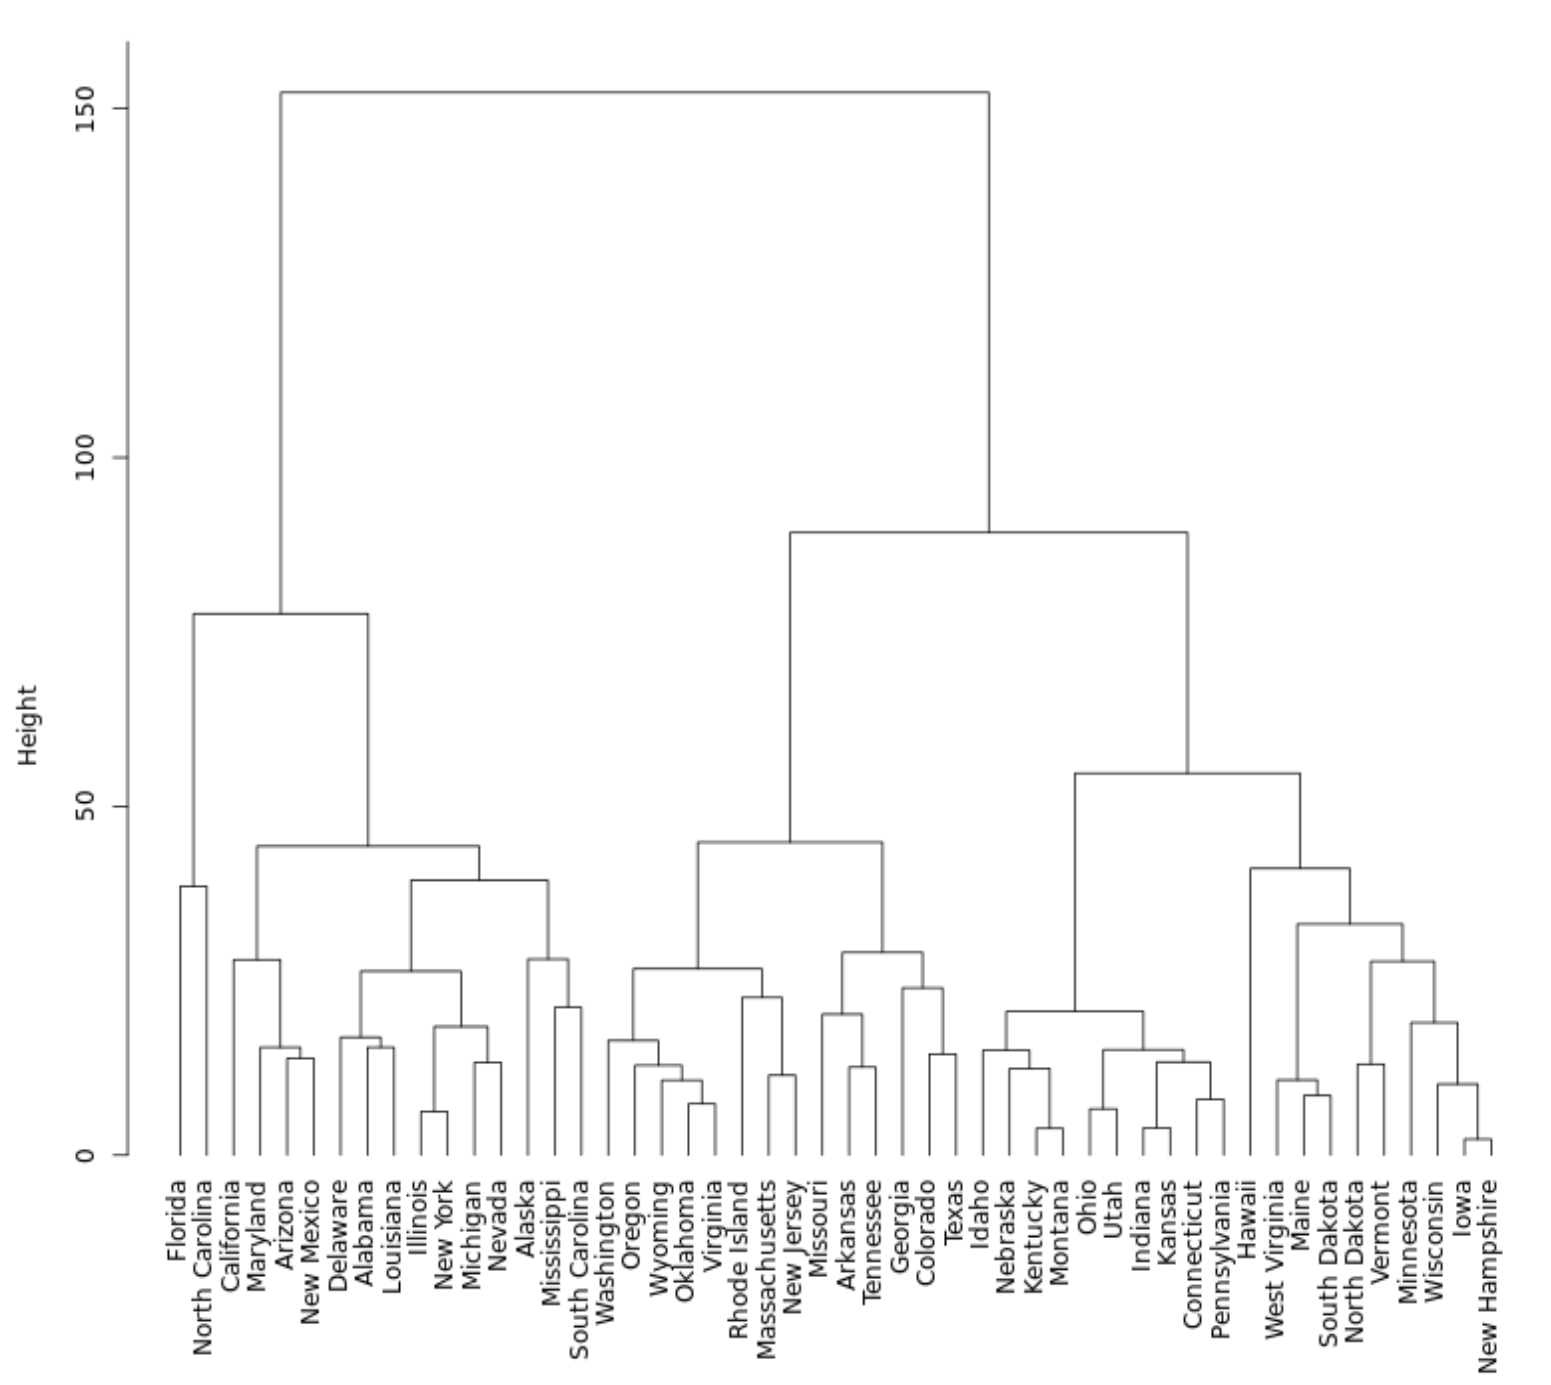
\includegraphics[width=10cm]{img/dendro}
	\caption{An example of a dendrogram; a plant growth under different treatment conditions (R dataset \texttt{PlantGrowth}).}
	\label{fig01:dendro}
\end{figure}

Hierarchical algorithms use two approaches on how to create a dendrogram; \emph{agglomerative} and \emph{divisive}. An agglomerative hierarchical algorithm begins with each object representing a cluster on its own. Then, in a bottom-up fashion, clusters are successively connected into the only cluster. The divisive algorithm begins with a single all-inclusive cluster which is divided into sub-clusters until single objects remain~\cite{rokach2005clustering}. 



To know which two clusters are connected (or respectively, how a cluster is~divided into two), algorithms use a \emph{dissimilarity measure} between clusters.  

\begin{defn}[Dissimilarity measure]
	Given a vector-space dataset $\mathcal{D}\subset\R^d$,  we define the \emph{dissimilarity measure} as the pair $(M,L)$. $M$ is a metric over $\R^d$ and $L$ is a linkage criterion; a function that can measure dissimilarity of subsets of $\R^d$ using $M$. They are used to measure the dissimilarity of clusters during a $\mathcal{D}$ clustering.
\end{defn}

A~hierarchical clustering model distinguishes various kinds of algorithms based on~the~choice of a metric and a linkage criterion. A \emph{distance function} can serve as a metric in a dissimilarity measure:

\subsubsection{Distance functions}

A distance function is used on objects of a dataset to measure how far they are from each other in the observed domain. For objects from a vector-space dataset, variations of \emph{Minkowski distance formula} (see eq.~\ref{eq01:mink}) can be used to easily create the metric for a dissimilarity measure.
They are \emph{Manhattan distance} ($p=1$), \emph{Euclidean distance} ($p=2$) and \emph{Chebyshev distance} ($p \to \infty$) (see tab.~\ref{tab01:mink}). The other possible metric is the \emph{cosine similarity} (see eq. \ref{eq01:cos}).

\begin{equation}\label{eq01:mink}
||a-b||_p = (\sum_{i=1...d}|a_i-b_i|^p)^{\frac{1}{p}}
\end{equation}

\begin{equation}\label{eq01:cos}
cos(a,b) = \dfrac{a\cdot b}{||a||||b||}
\end{equation}

As the choice of a distance function influences the result of a clustering, it should be chosen with respect to the properties of a provided dataset. \citet{aggarwal2001surprising} show the qualitative behavior of different distance functions in the $k$-means algorithm.



\begin{table}[t]
	\centering
	\renewcommand{\arraystretch}{1.3}
	\begin{tabular}{ll}
		\toprule
		Distance measure & Formula \\
		\midrule
		Manhattan & $\|a-b\|_1 = \sum_{i}|a_i-b_i|$          \\
		Euclidean & $\|a-b\|_2 = \sqrt{\sum_{i}(a_i-b_i)^2}$ \\
		Chebyshev & $\|a-b\|_\infty = \max_{i}|a_i-b_i|$  \\
		\bottomrule
	\end{tabular}
	\caption{Variations of the Minkowski distance formula.}
	\label{tab01:mink}
\end{table}

\subsubsection{Linkage criteria}

A~hierarchical algorithm can not compute the dissimilarity of two clusters only by a distance function; it is a function of dataset objects. To completely define the dissimilarity measure, we need a function of sets of object --- a linkage criterion. It describes any process of measuring dissimilarity between two groups of objects. In a hierarchical algorithm, it measures clusters to determine which two will be linked together. Given clusters $A$ and $B$ of a vector-space dataset and a distance function~$d$, we define the following linkage criteria~\cite{yim2015hierarchical} (see fig.~\ref{fig01:link}):

\begin{description}
	\item[Single linkage] -- The single linkage criterion computes the distance between $A$ and $B$ as the minimum distance between all pairs $(a,b) \in A\times B$:
	$$\min\{d(a,b) : a \in A, b \in B\}.$$
	
	The major drawback this criterion suffers is the \emph{cluster chaining}. It occurs when connected clusters do not share any other pair of close objects than the one that determined the connection. This produces long thin clusters with a big distance between some objects.
	
	\item[Complete linkage] -- The complete linkage criterion is similar to the single linkage criterion. But as opposed to~finding the minimum, this criterion uses the maximum of object pairs for the~computation of a cluster dissimilarity:
	$$\max\{d(a,b) : a \in A, b \in B\}.$$
	
	The criterion suffers from its simplicity as well as the single linkage. But~instead of naively connecting dissimilar clusters, here similar clusters are~not connected in some cases. Having all object pairs in a close proximity to each other but one object being rather far from the others, the~criterion will not link the clusters as the maximum distance deteriorates the rest.
	
	\item[Centroid linkage] -- The centroid linkage criterion tries to solve the problems of~the~aforementioned criteria by measuring the distance between the centroids of clusters. It~introduces a form of an average into the computation; the think that the criteria above lack.
\end{description}

The choice of a linkage criterion in hierarchical clustering algorithm is vital. As~stated above, it can change the course of clustering in a great manner. Chosen improperly, it can have a disastrous effect on the final result.

\begin{figure}\centering
	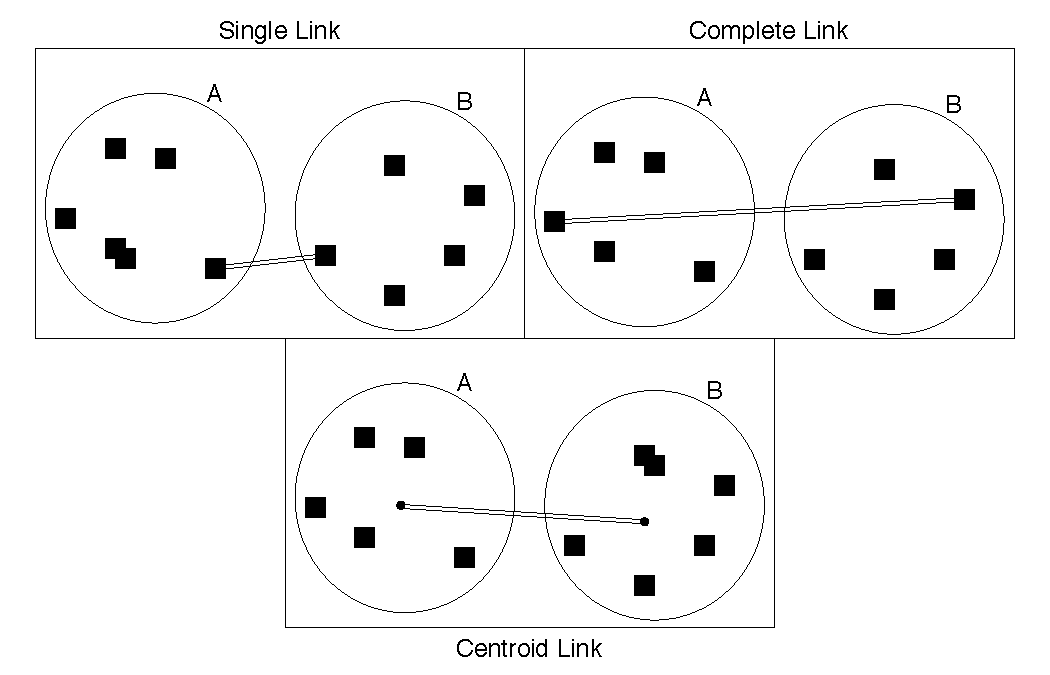
\includegraphics[width=10cm]{img/linkage_criteria}
	\caption{An example of three linkage criteria. The double line represents the~distance between clusters A and B according to the respective criterion.}
	\label{fig01:link}
\end{figure}

\section{Hierarchical clustering with Mahalanobis linkage}

\xxx{In} hierarchical clustering analysis (HCA)\todo{tady je uz ponekud pozde na zkratku}, algorithms branch into different variations so they are more suitable for a specific dataset type~\cite{murtagh2008hierarchical} \cite{oh2004hierarchical} \cite{zhao2005hierarchical}\todo{slep to do jednoho cite commandu, normalne cite\{a,b\} bez mezery}. \xxx{As an example of this process,} see fig.~\ref{fig01:mhca}\todo{ctenar se tam v tomhle okamziku podiva a nebude mu vubec jasny co tam ma hledat. Chces zacit tim ze typickej pripad pro podobnou customizaci je ze ocekavas urcitej tvar clusteru, napriklad ze jsou to pomerne dlouhy elipsoidy nebo gaussiany}. A general HCA is unable to properly cluster the \xxx{provided} dataset. The~\emph{Ma\-ha\-la\-no\-bis-average hierarchical clustering analysis} (MHCA) focuses on the datasets that create clusters of ellipsoid shapes. Such datasets are common \xxx{products}\todo{commonly originate in ...}\ of~the~measurements of cell cytometry data in bioinformatics, which was the original purpose for \xxx{its} design.

\begin{figure}[t]\centering
	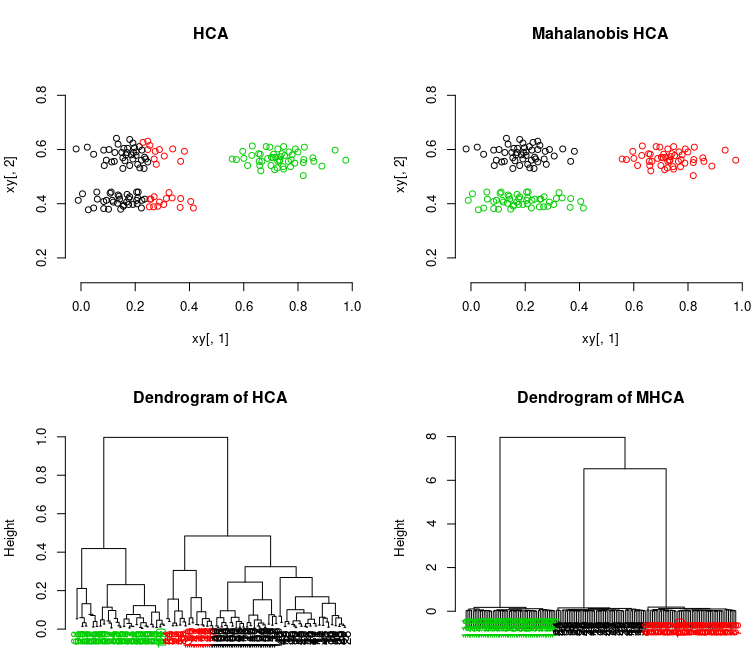
\includegraphics[width=10cm]{img/mhca}
	\caption{A comparison of HCA and MHCA clustering on a dataset that \xxx{forms} elliptic groups of points~\cite{fivser2012detection}. \xxx{je nutny rict odkud si vzal ten obrazek!} The upper two figures show the state of clustering when both algorithms cluster the dataset into three clusters. MHCA properly recognizes the elliptic clusters.}
	\label{fig01:mhca}
\end{figure}

\subsection{Mahalanobis distance}

A \xxx{vital} part of the MHCA is its \xxx{unique} dissimilarity measure\todo{zbytecna veta, slep s nasledujici}. It is based on the \emph{Mahalanobis distance}~\cite{mahalanobis1936generalized}, a~distance between a~point and a set of points (in our case a cluster). If points in the set are strongly correlated in some axis, then points laying on this axis are closer to the set than points that are not; even if their euclidean distance to the center of the set is closer.

To measure the Mahalanobis distance, \xxx{the} covariance matrix of~a~participating cluster needs to be computed. We \xxx{create} the covariance matrix using the random vector of a cluster.

\begin{defn}[Random vector of a cluster]
	Given a cluster $C$ of a vector-space dataset, we define its random vector $v$ as a vector of $d$ discrete random variables, where the random variable $v_i$ takes values from $\{x_i:x\in C\}$ with equal probability.
\end{defn}

\begin{defn}[Covariance matrix]
	Having a \xxx{random vector $v$ of length $n$}\todo{neni to set of vectors?!}, we define the \emph{covariance matrix} $\cov(v)$ as a $n\times n$ matrix that holds covariances of each pair of vector element:
	$$\cov(v)_{i,j}=\cov(v_i,v_j)$$
\end{defn}

Using the random vector of a cluster we can \xxx{easily create}\todo{neni to easily, a ty ji nevyrabis ale pocitas}\ the covariance matrix of a cluster and properly define the Mahalanobis distance:

\begin{defn}[Mahalanobis distance]
	Having a cluster $C$ of a vector-space dataset $\mathcal{D}\in\R^d$ and the random vector $v$ of $C$, we define the \emph{Mahalanobis distance} between $u \in \R^d$ and $C$ as
	\[d_\text{Maha}(u,C) = \sqrt{(u-\mean(C))^T\cov(v)^{-1}(u-\mean(C))}.\]
\end{defn}

\todo{Co se stane kdyz je $\cov(v)$ singularni?}

\xxx{However, using this equation,} we are only able to compute \xxx{a point cluster distance}. To fully incorporate the Mahalanobis distance in a hierarchical algorithm, we need to \xxx{find}\todo{construct?} a method \xxx{how} to measure a \xxx{cluster cluster distance}. 

\xxx{We can achieve it either by}\todo{rovnou rekni ze prirozene vznikaji 2 pouzitelny metody}\ computing the arithmetic mean of the distances between all points and a cluster or by computing just one distance between a centroid and a cluster. We respectively call these distance functions the \emph{Full Mahalanobis distance} (FMD) and the \emph{Centroid Mahalanobis distance} (CMD).

\begin{defn}[Full Mahalanobis distance]
	Having clusters $C$ and $C'$, we define the \emph{Full Mahalanobis distance} between clusters $C$ and $C'$ as the arithmetic mean of the Mahalanobis distances between each object $o \in C$ and the~cluster $C'$:
	$$d_\text{MahaFull}(C,C') =\frac{1}{|C|}\sum_{o\in C}{d_M(o,C')}$$
	\label{def01:fmd}
\end{defn}

\begin{defn}[Centroid Mahalanobis distance]
	Having a cluster $C$ with its centroid $c$ and a cluster $C'$, we define the \emph{Centroid Mahalanobis distance} between clusters $C$ and $C'$ as the Mahalanobis distance between $c$ and $C'$:
	$$d_\text{MahaCentroid}(C,C')=d_\text{Maha}(c,C')$$
	\label{def01:cmd}
\end{defn}


To illustrate the measure of the Mahalanobis distance, let us suppose we have two elliptic clusters. In the means of the proximity, the measure favors such clusters that their ellipsis are alongside rather than in a prolongation of one another~\cite{dagnelie1991using} (see fig.~\ref{fig01:ellipses}). Only when the objects of a cluster form a spherical shape, this measure of dissimilarity is proportional to the euclidean distance with a corresponding linkage.

\begin{figure}\centering
	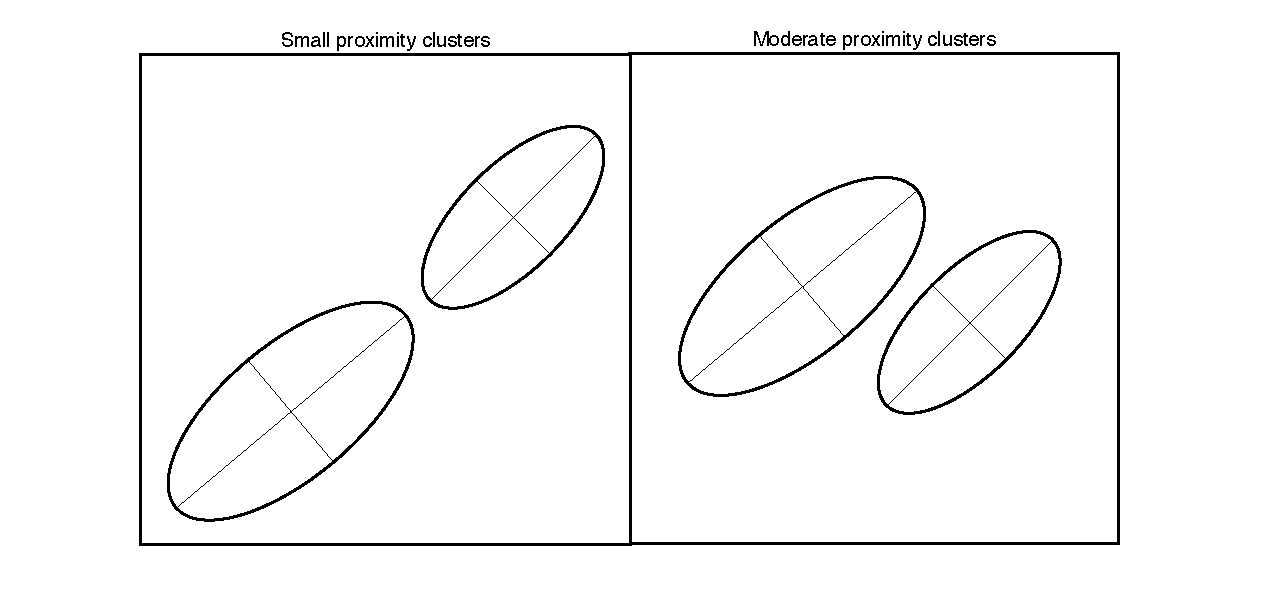
\includegraphics[width=10cm]{img/ellipses}
	\caption{An example of the cluster dissimilarity in the Mahalanobis-average hierarchical clustering.}
	\label{fig01:ellipses}
\end{figure}



The \xxx{pros and cons} between FMD and CMD are \xxx{trivial}. Due to the \xxx{full point contribution}\todo{def?}, FMC can produce more precise measure than its simpler counterpart. On the~other hand, CMD compensates this with much lower time complexity.\todo{jaky je meritko ty presnosti? V jakym pripade je teda presnost potreba, a kdy neni a vyplati se to aproximovat tim prumerem?}

To \xxx{make use of these} Mahalanobis distance variants in \xxx{MHCA} implementations, we need the distance function to be symmetric. Originally, the Mahalanobis distance is not a symmetric function. Fortunately, we easily fix the aforementioned distance functions with the \emph{Generalized distance}.

\begin{defn}[Generalized distance]
	Given clusters $C$, $C'$ and a variant of the Mahalanobis distance~$d_\text{Variant}$ (either FMD or CMD), we define the \emph{Generalized distance} between clusters $C$ and $C'$ as the arithmetic mean of distances between $C$, $C'$ and $C'$, $C$:
	$$d_\text{General}(C,C') = \frac{d_\text{Variant}(C,C')+d_\text{Variant}(C',C)}{2}$$
	\label{def01:gene}
\end{defn}  


\subsection{Algorithm behavior improvements}
\todo{Zlepsit nadpis, zabejvas se tady vylozene tim ze `Fixujes singularitu kovariancni matice'}

If the distance function of a MHCA implementation \xxx{was let to be the pure Mahalanobis distance, it would eventually halt due to the following problem --- the~covariance matrix computation.}

In early stages of MHCA --- when clusters consist of fewer points --- the covariance matrix of a cluster is often singular\todo{to je jeste v pohode protoze to dokazes detekovat, horsi je kdyz je `nearly singular' a zacnou ti vychazet vzdalenosti co se blizej}. Hence, we can not compute its inverse and perform the distance measure. Furthermore, the matrix can happen to be close to singular and --- when inverted --- can produce \xxx{distorted}\todo{specifikuj}\ results.

To solve this problem, \xxx{we used}\todo{Fiser et al used}\ the~euclidean distance with the~centroid linkage on clusters whose sizes are under a~specified threshold \xxx{--- the~\emph{Mahalanobis threshold}}. The value of the threshold is proportional to the size of a dataset~\cite{fivser2012detection}. \xxx{Hence,} to implement this optimization\todo{je to fakt optimalizace? neni to spis workaround?}\ we defined the \emph{Altered general distance}.\todo{eeeeeeeeeeeeeeemph}

\begin{defn}[Altered general distance]\todo{mozna by mnohem lepsi nazev byl `Non-singular Mahalanobis Distance' nebo tak neco}
	Given a threshold $T_M$, a cluster $C$ and its centroid $c$, a cluster $C'$ and its centroid $c'$ and a variant of the Mahalanobis distance~$d_\text{Variant}$ (either FMD or CMD), we define the \emph{Altered general distance} as
	$$
	d_\text{Altered}(C,C')=
	\begin{cases}
		d_\text{General}(C, C'),                       & \text{if $|C|\ge T_M$ and $|C'|\ge T_M$}, \\
		\dfrac{d_\text{Variant}(C, C')+||c-c'||_2}{2}, & \text{if $|C| < T_M$ and $|C'|\ge T_M$},  \\
		\dfrac{||c-c'||_2+d_\text{Variant}(C', C)}{2}, & \text{if $|C|\ge T_M$ and $|C'|< T_M$},   \\
		||c-c'||_2,                                    & \text{if $|C|< T_M$ and $|C'|< T_M$}.
	\end{cases}
	$$
	\label{def01:alt}
\end{defn}



\section{Computational complexity of the hierarchical clustering algorithms}

The common problem in clustering algorithms is their time complexity. In general, the time complexity of an agglomerative HCA is $O(n^3)$, which restricts \xxx{their} use for large datasets ($\geq10^5$ points \xxx{for} the contemporary hardware)~\cite{sasirekha2013agglomerative}.
A MHCA algorithm implementation \xxx{must be created with respect} to this problem. \citet{day1984efficient} propose three different variants of a \xxx{hierarchical clustering analysis}. We describe them thoroughly and \xxx{research}\todo{spis review, ale tu vetu asi muzes uplne vynechat (a pristi muzes slepit s predchozi)} their advantages and disadvantages.

The authors distinguish between three HCA algorithms based on the data structures they utilize:
\begin{itemize}
	\item HCA with the dissimilarity matrix,
	\item HCA with the nearest neighbor array,
	\item HCA with priority queues.
\end{itemize}

\subsection{HCA with the dissimilarity matrix}

\xxx{The first and the most trivial} variant uses the \emph{dissimilarity matrix} $M$.\todo{zbytecna veta}

\begin{defn}[Dissimilarity matrix]
	\xxx{Suppose} a dataset $\mathcal{D}$ divided into clusters $C_1,\dots,C_m$ and a function $d$ as a measure of dissimilarity. Then, the~\emph{dissimilarity matrix} $M$ is $m\times m$ matrix where $M_{ij} = d(C_i,C_j)$.
	\label{def01:dismat}
\end{defn}

Unless there remains only one cluster, the \xxx{current} algorithm searches $M$ for~the~closest pair of clusters\todo{bacha, pouzivas `closest' coz je distance na podobnost, kde chces `most similar', a zaroven bys mel upozornit na to ze `most similar' clustery se poznaj jako minimum v ty matici}, stores the pair and updates $M$ (see alg.~\ref{alg01:dismat}).

\begin{algorithm}[t]
	\caption{HCA with dissimilarity matrix}
	\label{alg01:dismat}
	\begin{algorithmic}[1]
		\Procedure{dismat}{$\mathcal{D} \subset \R^d$}
		\State initialize the dissimilarity matrix $M$
		\For{$k=|\mathcal{D}| \dots 1$}
		\State search $M$ for the closest pair $(i,j)$ \Comment{time: $O(k^2)$}
		\State store cluster pair $(i,j)$ into the merge list \Comment{time: $O(1)$}
		\State update $M$ \Comment{time: $O(k)$}
		\EndFor
		\State \textbf{return} list of merged clusters
		\EndProcedure
	\end{algorithmic}
\end{algorithm}

The main cycle \xxx{in}\todo{on?}\ line $3$\todo{tady nastava zmateni protoze ctenar netusi kde ma vzit ten treti radek, idealne tohle chces ve stejnym odstavci jako referenci na ten algoritmus, tak aby bylo videt ze ty radky sou z nej} repeats $n = |\mathcal{D}|$ times; \xxx{each iteration}\todo{predlozku?}\ the number of clusters is reduced by 1. The search in line $4$ is bounded by $O(n^2)$ time, \xxx{having its peak}\todo{with maximal complexity}\ in the first iteration when $k=n$. The update in~line~$6$ reflects the deletion of clusters $i$ and $j$ and the addition of the new one. Hence, it needs to perform $k$ new dissimilarity measur\xxx{es}\todo{measurements?}\ for the new cluster (bounded by $O(n)$ during the first iteration as well). As there are total $n$~iterations performed, this results in the overall time complexity of $O(n^3)$. 

The space required to store $M$ is $O(n^2)$. As there is no other non-trivial requirement, the overall space complexity is $O(n^2)$ as well.

\todo{Z tech poznamek udelej oddeleny algoritmy, kdyz uz maj uplne jinou slozitost tak je dobry to videt explicitne. Zaroven se tim definuje ten `In-place HCA' kterej mas v tabulce ale tady neni nikde videt.}
\begin{rem}
	Note that this algorithm does not have to store the dissimilarity matrix in the memory. We can decide to measure a cluster dissimilarity \emph{in-place}. Line $6$ would become redundant and the time complexity of line $4$ would increase by a constant multiplicative factor; hence, the overall time complexity remains the same while the~space complexity becomes $O(n)$. We will refer to this variant as the \emph{in-place HCA}.
\end{rem}


\subsection{HCA with the nearest neighbor array}
This algorithm introduces the array of the nearest neighbors.

\begin{defn}[Nearest neighbor array]
	Suppose a dataset $\mathcal{D}$ divided into clusters $C_1,\dots,C_m$ and a function $d$ as a measure of dissimilarity. Then, the~\emph{nearest neighbor array} $N$ is a $m$-element array of indices $\{1,\dots,m\}$ such that for each element $N_i$ holds
	$$d(C_i,C_{N_i}) = \min\{d(C_i,C_j) : j \in \{1,\dots,m\} \setminus \{i\}\}$$
	\label{def01:neigh}
\end{defn}

Instead of the dissimilarity matrix, each cluster is assigned the index pointing to~its closest neighboring cluster. 
Compared with the previous algorithm, this algorithm trades the expensive \emph{closest pair search} with the expensive \emph{structure update}  (see alg.~\ref{alg01:neigh}).



\begin{algorithm}[t]
	\caption{HCA with the nearest neighbor array}
	\label{alg01:neigh}
	\begin{algorithmic}[1]
		\Procedure{neighbor}{$\mathcal{D} \subset \R^d$}
		\State initialize $N$
		\For{$k=|\mathcal{D}|\dots 1$}
		\State search $N$ for the closest pair $(i,j)$ \Comment{time: $O(k)$}
		\State store cluster pair $(i,j)$ into the merge list \Comment{time: $O(1)$}
		\State update $N$ \Comment{time: $O(k^2)$}
		\EndFor
		\State \textbf{return} list of merged clusters
		\EndProcedure
	\end{algorithmic}
\end{algorithm}


In line $4$, each closest pair search can be performed in $O(n)$ time as the~array length does not exceeds $n$ elements. However in line $6$, the worst case update of $N$ happens when each cluster resides in the closest neighborhood with the clusters that are being merged (clusters $i$  and $j$). In this case, the~whole array has to be recomputed, which corresponds to~the~computation of the whole dissimilarity matrix. Hence, the time complexity for~this step is $O(n^2)$. To sum up, the overall time complexity is $O(n^3)$ and~the~space complexity is $O(n)$ because $N$ does not have more than linear space requirements.

Despite the equal time complexities, this algorithm may outperform the previous one because in the majority of situations the update step in line $6$ does not require the whole array to be recomputed. Moreover, if the~number of elements to be updated remains constant each iteration, the overall algorithm time complexity may be $O(n^2)$. 

\subsection{HCA with priority queues}

This algorithm takes the advantage of the previous one employing the fast search and combines it with the fast update using \emph{priority queues} (see alg.~\ref{alg01:queue}).
Each object from a dataset is assigned a~priority queue constructed from the remainder of the dataset. The priority label of a queued element is a dissimilarity measure between the object and the queued element. 

\begin{algorithm}[t]
 	\caption{HCA with priority queues}
 	\label{alg01:queue}
 	\begin{algorithmic}[1]
 		\Procedure{queues}{$\mathcal{D} \subset \R^d$}
 		\ForAll{$o \in \mathcal{D}$}
 		\State initialize a priority queue from $\mathcal{D} \setminus \{o\}$
 		\EndFor
 		\For{$k=|\mathcal{D}|\dots 1$}
 		\State search $k$ queues for the closest pair $(i,j)$ \Comment{time: $O(k)$}
 		\State store cluster pair $(i,j)$ into the merge list \Comment{time: $O(1)$}
 		\State update $k-1$ priority queues \Comment{time: $O(k\log{k})$}
 		\EndFor
 		\State \textbf{return} list of merged clusters
 		\EndProcedure
 	\end{algorithmic}
\end{algorithm}

When a priority queue is implemented as a heap, its time complexity can be $O(1)$ for the minimum retrieval and $O(log(n))$ for the insertion and deletion of an element~\cite{fredman1987fibonacci}.
Therefore, the search step in line $4$ takes $O(k)$ time (bounded by~$O(n)$ during the first iteration). Next in line $6$, we need two delete and one insert operations (corresponding to deleting two merged clusters and inserting one new). We can perform such update on $n$~queues in $O(n\log{n})$ time.

To sum up, the overall time complexity is $O(n^2\log{n})$. The space complexity is $O(n^2)$ because all $n$ queues have the linear space requirements.

\vspace{0.5cm}

We summarize the time and space complexity of the mentioned algorithms in the table~\ref{tab01:hca}.

\begin{table}[t]
	\centering
	\begin{tabular}{lcc}
		\toprule
		 & \textbf{Time} & \textbf{Space} \\
		 \pulrad{\textbf{HCA variant}} & \textbf{complexity} & \textbf{complexity} \\
		\midrule
		HCA with dissimilarity matrix & $O(n^3)$ & $O(n^2)$ \xxx{mathcal O!}\\
		in-place HCA & $O(n^3)$ & $O(n)$ \\
		HCA with the nearest neighbor array & $O(n^3)$ & $O(n)$ \\
		HCA with priority queues & $O(n^2\log(n))$ & $O(n^2)$ \\
		\bottomrule
	\end{tabular}
	\caption{The summary of time and space complexity for the HCA variants. \xxx{Tohle je trochu nepresny --- neni v tom videt zavislost na slozitosti vypoctu ty disimilarity (tj. efektivne na dimenzionalite toho datasetu). Doporucuju to udelat aspon pro ty minkowskiho vzdalenosti tim ze tam pridas vliv ty dimenze. Konkretne v prvnim radku ma bejt $\mathcal{O}(n\cdot(n^2 + nd))$ (coz ma vyhodu pro obrovsky $d>>>n$) a v druhym to je na ferovku $\mathcal{O}(n^3\cdot d)$}}
	\label{tab01:hca}
\end{table}

To show an example of the big algorithm complexity, we tested the limits of a dissimilarity matrix variant implementation. We measured the R language library function \texttt{hclust}; a frequently used implementation of HCA. It computes the centroid linkage with the euclidean distance and uses the dissimilarity matrix. 

Fig. \ref{fig01:hclust} confirms the above stated polynomial time complexity of the implementation. Moreover, it halted at a dataset size of 47K because the testing machine \footnote{Intel Core i9-8950HK, 32GB RAM} ran out of memory.

In conclusion, the space complexity of HCA can be even more restrictive in the means of the overall algorithm usability than its time complexity. The performance and usability of the HCA variants depends on many factors and the programmer needs to find a balance between their tradeoffs. The metric function is one of them. For example, when the Minkowski distance is used, we can prefer the in-place HCA over the HCA with dissimilarity matrix for a lower space complexity while retaining the same asymptotic time complexity. However, if the distance metric is more complex, one may prefer to store the measures in the memory.

\begin{figure}\centering
	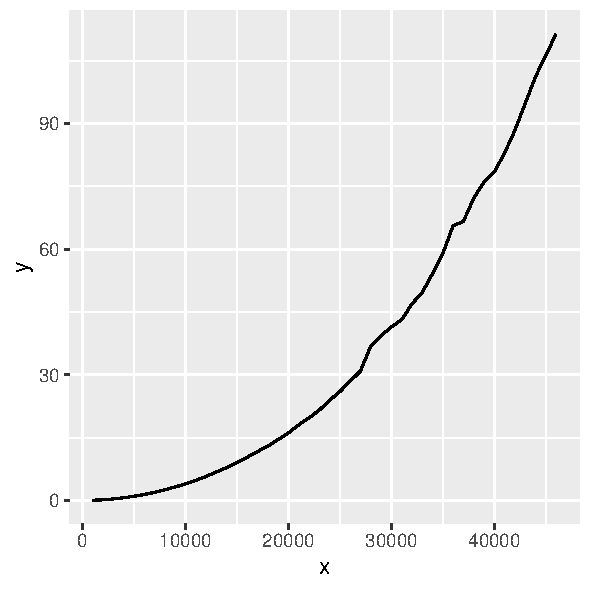
\includegraphics[width=10cm]{img/hclust}
	\caption{Time complexity of \texttt{hclust} with respect to the size of a dataset.}
	\label{fig01:hclust}
\end{figure}

\chapter{GPU implementation}

This chapter guides the reader through the implementation of Mahalanobis-based hierarchical clustering analysis. First, we describe the algorithm and high level look on implementation. Then, we thoroughly describe the most important functions.

\section{The Algorithm}

The first chapter introduced three views on implementation of hierarchical clustering. To decide which one to choose we need to take into account two major conditions. First, the algorithm shall not require quadratic \emph{space complexity} as it must be able to process rather large datasets. Second, the algorithm should exhibit some \emph{parallelism opportunities}; otherwise massive GPU parallel properties will be to no use.  We describe mentioned algorithms according to this conditions:
\begin{description}

\item[HCA with dissimilarity matrix] satisfies the first condition if the dissimilarity matrix will not be held in the memory. The second condition is satisfied as each matrix field can be computed independently exposing great parallelism opportunity. 

\item[HCA with the nearest neighbor array] is required sub-quadratic space complexity by definition. On the other hand, it provides less means of parallelism as the algorithm need not compute whole dissimilarity matrix as in the previous algorithm. However, large datasest sizes may compensate for this disadvantage. 

\item[HCA with priority queues] is unusable as it does not satisfy the first condition. Moreover, operation over priority queues (insert, delete and min) are not of a parallel nature and may create bottleneck in the computation.

\end{description}

For this thesis we chose to implement HCA with the nearest neighbor array. It promises better time complexity than the HCA with dissimilarity matrix which can come to a great use when clustering big datasets. In addition, we utilized the advantages of priority queues by defining a constant that declares the number of closest neighbors assigned to each cluster.

Additionally, we chose to implement the CMD variant of Mahalanobis distance to fully exhibit GPU parallel properties.

\subsection{Apriori clusters}

When cluster sizes reach the Mahalanobis threshold, a MHCA algorithm starts to form elliptic shaped clusters. However, until then, simple euclidean distance is used. This is an important stage of the algorithm as an improper initial clustering can decrease the overall clustering result. Hence, a simple hierarchical euclidean clustering can be unsatisfactory.

To solve this problem, we implemented additional feature to the algorithm called \emph{apriori clusters} (see def. \ref{def03:apriori}). The intended usage of the feature is that the apriori clusters are created from a dataset using non-hierarchical clustering algorithm such as \emph{k-means} --- the algorithm that would be capable of creating better initial clusters that a MHCA algorithm. 

With this, a MHCA algorithm is guided by the apriori clusters to create plenty of small clusters that just reached the Mahalanobis threshold; these clusters can now fully exhibit the MHCA properties. Overall, we suppose that we can lessen the probability of an error during the early stage of the algorithm.

\begin{defn}
	Suppose a dataset $\mathcal{D}$, a HCA algorithm $\mathcal{A}$ and a partitioning of  $\mathcal{D}$ into non-empty subsets $a_1,\dots,a_k$. If following conditions hold:
	\begin{enumerate}
		\item $\mathcal{A}$ performs clustering of each subset separately. Meaning that clusters from different subsets can not be merged.
		\item When each subset is clustered into the only cluster, $\mathcal{A}$ clusters the resulting clusters as if they were in one subset.
	\end{enumerate}
	then we call the subsets $a_1,\dots,a_k$ \emph{apriori clusters} of $\mathcal{A}$.
	\label{def03:apriori}
\end{defn}

\section{The algorithm implementation}

The above mentioned algorithm is implemented in the main class of the program --- \texttt{gmhc}\footnote{An abrevation for GPU Mahalanobis-based hierarchical clustering.}. It inherits from an abstract template class \texttt{hierarchical\_clustering}.

\subsection{Class \texttt{hierarchical\_clustering}}
This template provides key data fields and methods for a hierarchical clustering algorithm (see list. \ref{lst03:hc}): 

\begin{description}
	\item[\texttt{initialize()}] sets the fields of the class. A templated field \texttt{points} is an array of dataset objects --- points. They are expected to be of a floating-point numeric type. Fields \texttt{point\_dim} and \texttt{points\_size} state a point dimensionality and a total number of points in the array. Hence, each \texttt{point\_dim} consecutive array elements represent one point and the total array size being $\texttt{point\_dim}*\texttt{points\_size}$ elements.
	
	\item[\texttt{run()}] initiates the clustering. It returns a vector of \texttt{pasgn\_t} structures --- pairs that contain \emph{assignments} --- the IDs of merged clusters. Each point from the input array is assigned an unique consecutive ID starting from $0$. When two clusters are merged, the new cluster is assigned the next available unique ID. The process of merging is then stored in the returning vector. Hence, the vector completely describes the whole clustering process.
	
	\item[\texttt{free()}] deallocates all acquired resources.
\end{description}

\begin{lstlisting}[caption={A summary of \texttt{hierarchical\_clustering} header file.},label={lst03:hc}]
using csize_t = uint32_t;
using asgn_t = csize_t;
using pasgn_t = std::pair<asgn_t, asgn_t>;

template <typename T>
class hierarchical_clustering
{
protected:
	const T* points;
	csize_t points_size;
	csize_t point_dim;
public:
	virtual void initialize(...);
	virtual std::vector<pasgn_t> run() = 0;
	virtual void free() = 0;
};
\end{lstlisting}

\subsection{Class \texttt{gmhc}}

This class is the main entrypoint of the whole MHCA algorithm. It inherits from \texttt{hierarchical\_clustering<float>} template specialization, which means that the algorithm expects dataset objects to be single-precision points of a specified dimension. The class communicates
with a GPU; hence, it holds structures used by the device.

It contains an array of \texttt{clustering\_context\_t} objects. Each of them holds the context of a specific part of the dataset and is able to perform a clustering on it.

\subsubsection{Initialization}

Initialization happens in the \texttt{initialize} method. Due to the initialization of device and host structures, this stage must be treated with importance.
The class overloads \texttt{initialize} method so that it sets three additional fields:
\begin{itemize}
	\item \texttt{mahalanobis\_threshold} indicates the threshold in the \emph{Altered general distance} (see def. \ref{def01:alt}).
	
	\item\texttt{apriori\_assignments}  is an array of assignments that splits \texttt{points} into \emph{apriori clusters}. This is an optional field of the \texttt{initialize} method.
	
	\item \texttt{validator} is an optional field used for testing purposes.
\end{itemize}

Next follows the main responsibility of the \texttt{initialize} method --- device and host data allocation and initialization. Device data fields are prefixed with \texttt{cu\_}\footnote{Abbreviation for CUDA.} and are run within kernels. Host data control a flow of run kernels. They are mainly arrays that are organized in such a way that they can be cut into sub-arrays each managing context of one apriori cluster. They will be further described in the following sections.

\subsubsection{Clustering}
The clustering algorithm resides in the method \texttt{run}. This method utilizes the array of \texttt{clustering\_context\_t} objects. If \texttt{apriori\_assignments} are present, each element of the array contains context of a corresponding apriori cluster and holds methods for its further clustering. 

In addition to that, the method uses one special clustering context called the \emph{final context}. If apriori clusters are present (and the above mentioned array is not empty), it is unset and serves as a context that will host all the apriori cluster results for the final clustering. If there are no apriori clusers, the final context is set and contains the whole dataset.

We divide the whole clustering algorithm into a top level \emph{apriori clustering} and a low level \emph{context clustering}.

\begin{description}
	\item[Apriori clustering] handles a separate clustering of apriori clusters, merging their results into one clustering context and performing the final clustering (see alg. \ref{alg03:apriori}).
	
	The algorithm iterates over each apriori clusters from the context array. It perfroms its clustering and the result is inserted into the final context. Either when all apriori clusters are merged or when there are none at all, the final context with the remaining clusters is clustered and the list of assignment pairs is returned.
	
	Before any context begins the clustering, its closest neighbor array has to be initialized. It is done by the kernel \texttt{run\_neighbors}.
	
	
	\begin{algorithm}
		\caption{Apriori clustering}
		\label{alg03:apriori}
		\begin{algorithmic}[1]
			\Procedure{apriori}{$\mathcal{C}, ctx_f$}
			\ForAll{$ctx \in \mathcal{C}\cup ctx_f$} \Comment{iterate over apriori clusters and the final context}
			\State initialize the closest neighbor array of $ctx$ \Comment{kernel \texttt{run\_neighbors}}
			\While{$ctx$ has not the only cluster}
			\State iterate clustering of $cxt$ for the closest pair $(i,j)$
			\State store $(i,j)$ into the returning list
			\EndWhile
			\State $ctx_f \gets ctx_f \cup ctx$ \Comment{assign merged cluster into the final context}
			\EndFor
			\State \textbf{return} list of merged clusters
			\EndProcedure
		\end{algorithmic}
	\end{algorithm}

	\item[Context clustering] is
	
	\begin{algorithm}
	\caption{Context clustering}
	\label{alg03:context}
	\begin{algorithmic}[1]
		\Procedure{apriori}{$\mathcal{C}, ctx_f$}
		\ForAll{$ctx \in \mathcal{C}\cup ctx_f$} \Comment{iterate over apriori clusters and the final context}
		\State initialize the closest neighbor array of $ctx$ \Comment{kernel \texttt{run\_neighbors}}
		\While{$ctx$ has not the only cluster}
		\State iterate clustering of $cxt$ for the closest pair $(i,j)$
		\State store $(i,j)$ into the returning list
		\EndWhile
		\State $ctx_f \gets ctx_f \cup ctx$ \Comment{assign merged cluster into the final context}
		\EndFor
		\State \textbf{return} list of merged clusters
		\EndProcedure
	\end{algorithmic}
\end{algorithm}

\end{description}





 

\chapter{Results}

The last chapter of the thesis describes the experiments that were performed to~provide a clear result of the MHCA implementation performance. The aim of~the~thesis was to create the MHCA implementation that is capable of clustering datasets of hundred thousands and millions of points in a reasonable amount of~time.

The results were compared with a different implementation of Mahalanobis-average hierarchical clustering \cite{fivser2012detection}. It is a R language implementation with performance critical parts written in C language. It provides both FMD and CMD measures of dissimilarity and the apriori clusters computation as well. It performs a~serial CPU computation. For brevity, we denote the thesis GPU implementation by \texttt{gmhclust} and the serial CPU version by \texttt{mhclust}.

The testing datasets were divided into these two categories:

\begin{description}
	\item[Single-point datasets] These datasets are clustered without a knowledge of any apriori clusters. Hence, the computing starts from a single point. The datasets are purely of a high-dimensional flow and mass cytometry data \cite{flowrepo} (see tab.~\ref{tab04:single}).
	
	\begin{table}
		\centering
		\begin{tabular}{lcc}
			\toprule
			\textbf{Dataset name} & \textbf{Size} & \textbf{Dimension} \\ \midrule
			\emph{Niellson\_rare} &      44K      &         14         \\
			\emph{Levine\_13dim}  &     167K      &         13         \\
			\emph{Levine\_32dim}  &     265K      &         32         \\
			\emph{Mosmann\_rare}  &     396K      &         15         \\
			\emph{Samusik\_all}   &     841K      &         39         \\ \bottomrule
		\end{tabular}
	\caption{Flow and mass cytometry datasets selected for experiments.}
	\label{tab04:single}
	\end{table}

	\item[Apriori datasets] These datasets are clustered with apriori clusters. They do not represent any measured data. Rather, for each dataset, a set of distinct clusters was artificially created for this purpose. Each cluster was randomly generated as a set of $d$-dimensional points with the normal distribution and evenly scattered among the dataset. The describing parameters of~apriori datasets are the \emph{apriori cluster size}, the \emph{apriori cluster count} and the \emph{point dimensionality} (see tab.~\ref{tab04:apriori}). To find the apriori clusters, they need not be pre-computed by another clustering algorithm (such as k-means) as~all the~points are already stored with respect to the apriori clusters.
	
	\begin{table}
		\centering
		\begin{tabular}{lcccc}
			\toprule
			\textbf{Dataset name} & \textbf{Cluster size} & \textbf{Cluster count} & \textbf{Size} & \textbf{Dimension} \\ \midrule
			\emph{apriori\_1M}    &         1000          &          1000          &      1M       &         20         \\
			\emph{apriori\_2M}    &         2000          &          1000          &      2M       &         20         \\ \bottomrule
		\end{tabular}
		\caption{Apriori datasets generated for experiments.}
		\label{tab04:apriori}
	\end{table}
	
\end{description}

All experiments were run on the same machine (Intel Xeon Silver 4110, 256 GB RAM, NVIDIA Tesla V100 PCIe 16 GB). The performance related experiments were performed several times. As there were negligible performance differences in the separate runs, all the following plots depicting performance show their arithmetic means. 

\section{The closest neighbor parameter}

To determine which clusters to merge, the GPU implementation uses the closest neighbor array. The number of the closest neighbors assigned to each cluster in~the~array is variable. We experimented on single-point and apriori datasets with this parameter to determine which number performs best. 

We assumed that \emph{two} closest neighbors will achieve the best performance as~it will result in the reduced number of cluster to be updated each iteration. \emph{Three} and more neighbors will not provide such reduction that would compensate the~diminishing returns caused by the longer time for a cluster update.

\begin{figure}\centering
	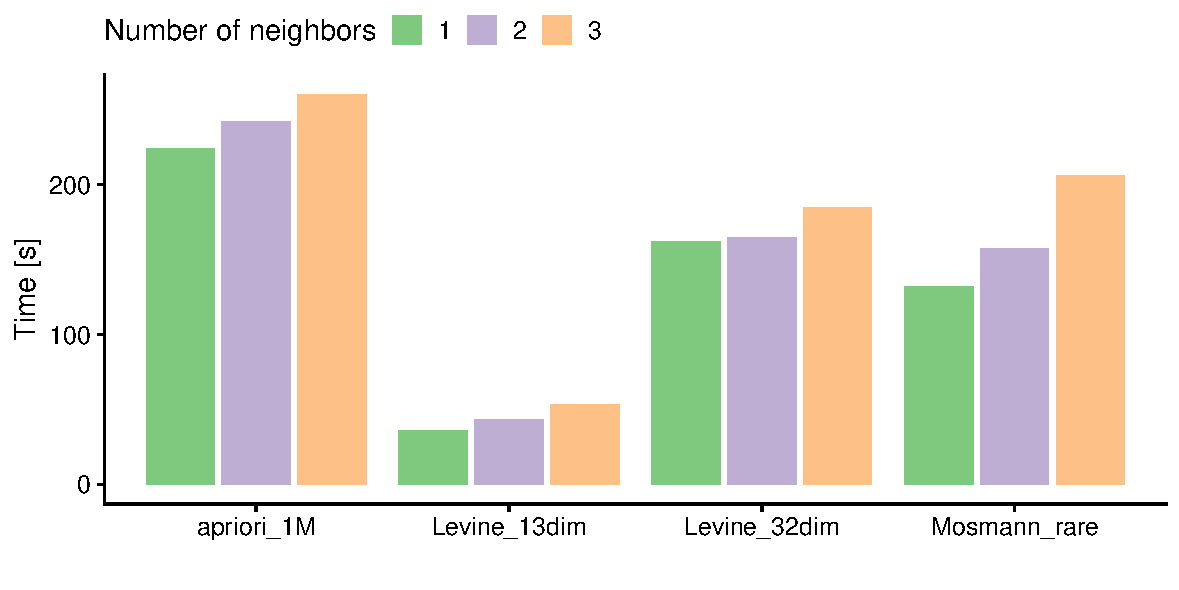
\includegraphics[width=\linewidth]{img/neighbor_compare}
	\caption{A comparison of \texttt{gmhclust} with various numbers of neighbors assigned to clusters.}
	\label{fig04:neigh}
\end{figure}

As can be seen from the figure \ref{fig04:neigh}, the variant of 1 closest neighbor achieved the~best performance. It may be caused by the fact that the lower number of cluster updates did not overcome the increased time for each update. Alternatively, it may be caused by the composition of tested datasets; datasets that naturally form cluster of other than elliptical shape may benefit better from another closest neighbor number variant.

The forthcoming experiments will be performed with the 1 closest neighbor variant.

\section{Performance speedup}

The next set of experiments determines the performance speedup of~the~GPU implementation over the CPU implementation. The performance comparison was performed on single-point and apriori datasets separately.

Unfortunately, during the single-point testing, we reached the computational limits of the CPU implementation. Even for the smallest dataset, the computation took nearly 14 hours. Due to the polynomial time complexity and extremely increasing memory requirements (193GB for Levine\_32), we decided that in order to test the datasets, we need to down-sample them. We uniformly randomly selected a fraction of the dataset points to create a smaller dataset. Note that these consequences are necessary (yet unforeseen) as the larger datasets require such big amount of time and space resources that they are by no means practically computable (see fig.~\ref{fig04:fract_comp}).

\begin{figure}\centering
	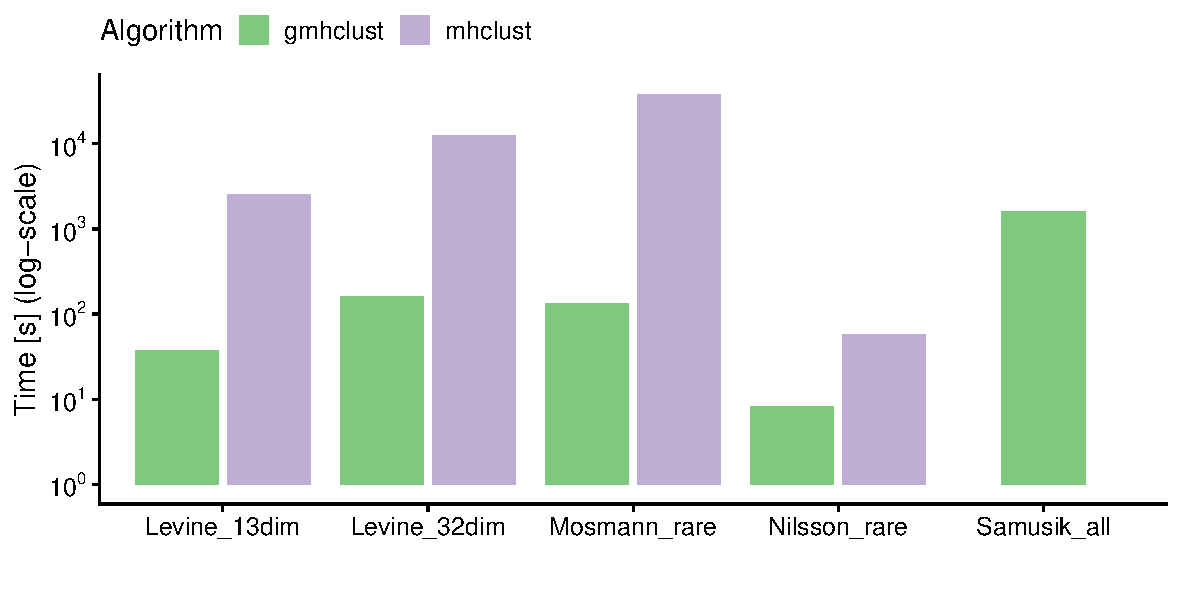
\includegraphics[width=\linewidth]{img/mixed_perf_comp}
	\caption{An example of a poor performance of \texttt{mhclust} compared with \texttt{gmhclust} on single-point datasets. Datasets of \texttt{mhclust} were down-sampled to the fraction of $\frac{1}{10}$ while \texttt{gmhclust} datasets were not changed. For Samusik\_all dataset, neither the fraction of $\frac{1}{10}$ did help to finish the computation within a 24 hours mark.}
	\label{fig04:fract_comp}
\end{figure}

\subsection{Single-point datasets performance speedup}

To determine the performance increase, we decided to down-sample Nillson\_rare dataset (as it is the smallest one). We created 10 samples with their sizes corresponding to 10\% of the dataset up to 100\%.
As seen from the figure \ref{fig04:single_perf}, the~performance difference increases as the~dataset size increases. It is a common consequence of~the~fact that there is less work to parallelize in smaller datasets than in~bigger datasets. In the dataset of size around 4K, the performance of \texttt{gmhclust} is 60-times greater. This scales up to 5000-times faster time for the full Nilsson\_rare dataset.

\begin{figure}\centering
	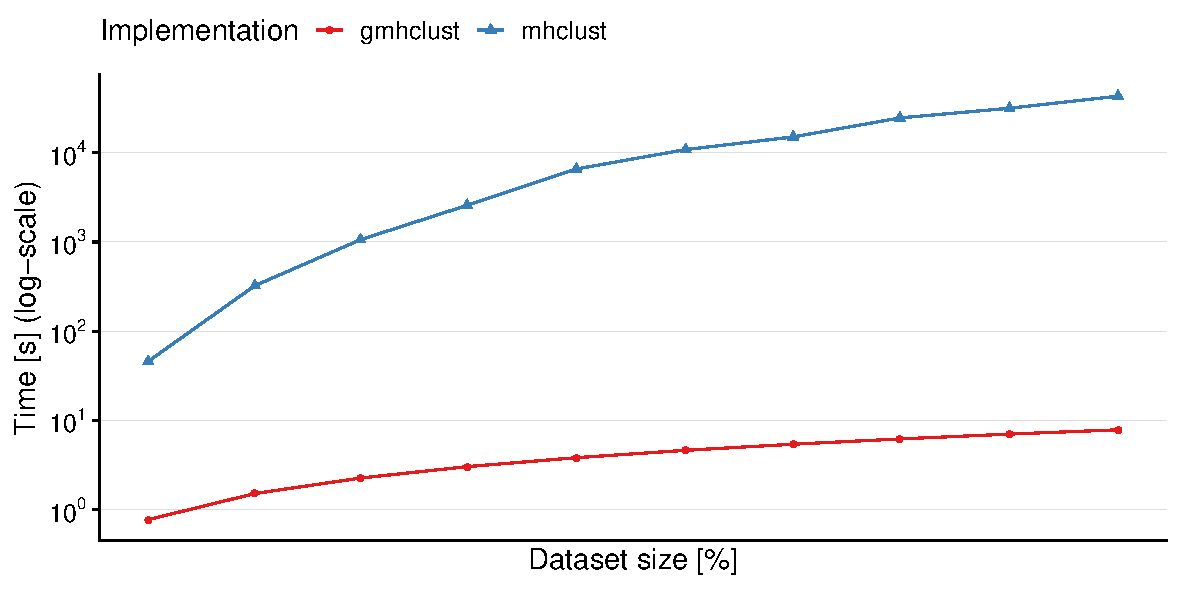
\includegraphics[width=\linewidth]{img/single_perf_comp}
	\caption{A comparison of \texttt{gmhclust} and \texttt{mhclust} performance on various sizes of Nilsson\_rare single-point dataset.}
	\label{fig04:single_perf}
\end{figure}

\subsection{Apriori datasets performance speedup}

In contrast with the single-point datasets, the CPU implementation managed to~compute apriori datasets of big sizes. It is a consequence of the wisely chosen apriori clusters.

When the algorithm is inputed with apriori clusters, it does not compute the~whole dataset at once --- it clusters each apriori cluster first. This fact reduces the overall time complexity significantly, allowing the CPU algorithm to compute big datasets in a short amount of time.

For example, suppose the input dataset apriori\_2M and a function $f$ that takes a dataset size and outputs the required time for its clustering. Then, the algorithm performance is proportional to $$1000f(2000)+f(1000)$$ that is --- deducing from the previous experiment --- far less than $f(1000\cdot 2000)$.

We measured the performance of the CPU and GPU implementation on apriori\_1M and apriori\_2M (see fig.~\ref{fig04:apr_perf_comp}). The results of the performance increase are~8-times and 20-times respectively. As we expected, it is not as measurable as~in~single-point datasets even though it has much more points. 

It is caused by computing a lot of small apriori clusters. From the previous experiment we observed that small-sized datasets do not exhibit such big increase in performance. Therefore, the overall performance increase in apriori datasets is not expected to be drastically better.

\begin{figure}\centering
	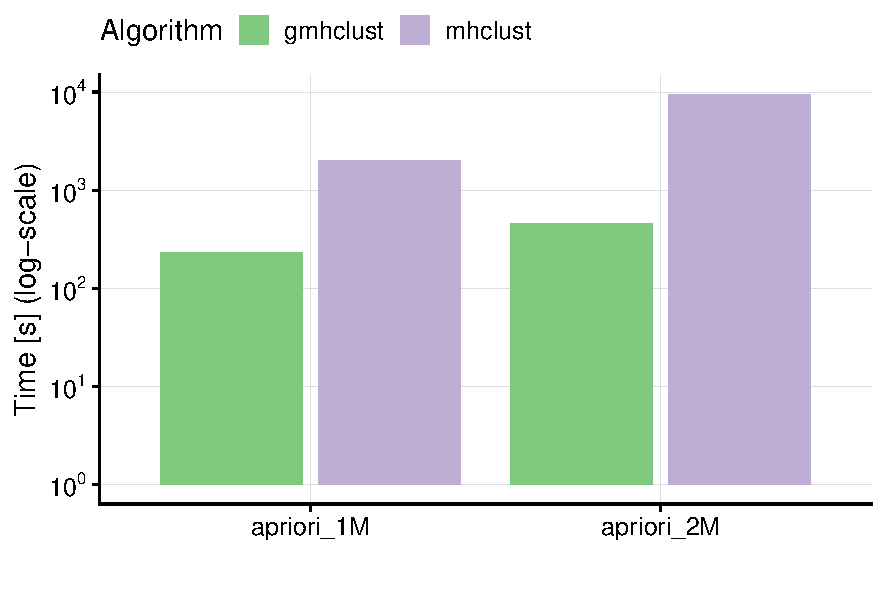
\includegraphics[width=10cm]{img/apriori_perf_comp}
	\caption{A comparison of \texttt{gmhclust} and \texttt{mhclust} on apriori datasets.}
	\label{fig04:apr_perf_comp}
\end{figure}

\subsubsection{Apriori dataset parameters}

The next experiment tests how the apriori dataset parameters \emph{size} and \emph{count} influence the overall algorithm time. We tested 7 different size--count ratios on~a~dataset of~5M 20-dimensional points (see fig.~\ref{fig04:apr_ratio}). The Mahalanobis threshold of each run was set to be equal to the apriori cluster size.

The runs are ordered in such way that the apriori cluster size is increasing (and the apriori cluster count is decreasing). The plotted line first rapidly decreases, then is close to constant and starts to increase in the end. This may be~caused by two factors:

First, according to the previous experiment, we expected the following relation: the bigger is the maximum of the size and count parameters, the bigger is~the~overall computational time. Hence, big measured values are seen on~the~edges of the plot. 

The second factor may be the Mahalanobis threshold. As the threshold increases with the increasing cluster size, more clustering work is performed using the less demanding euclidean distance. The threshold was set to be equal to~the~apriori cluster size; hence, the Mahalanobis distance is used after all apriori clusters are clustered. As the consequence, the right edge of the plot is~not as~steep as the left edge.

\begin{figure}\centering
	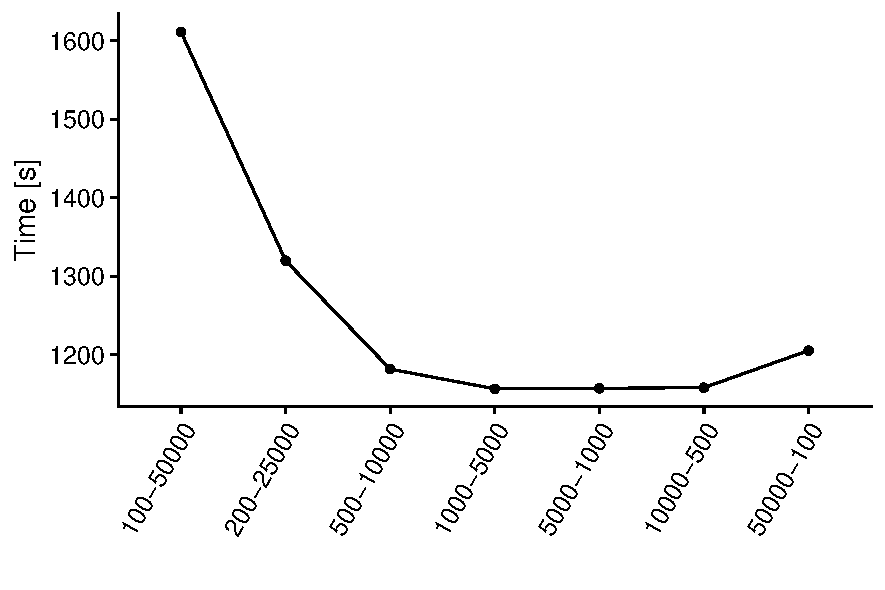
\includegraphics[width=10cm]{img/5M-compare}
	\caption{\texttt{gmhclust} performance for different ratios of apriori cluster size and count (depicted as $size$-$count$) with Mahalanobis threshold set to $size$.}
	\label{fig04:apr_ratio}
\end{figure}

\section{Results comparison}

Next, we will compare the clustering results of the GPU and CPU implementation to see if they are similar. Comparing results for equality would put big restrains on the implementation. Rather, we want to allow algorithms to have slight differences during their clustering and compare the whole clustering process. First, we need to define the \emph{point height}.

\begin{defn}[Point height]
	Suppose a dataset $\mathcal{D} \subset \R^d$  and an ordered sequence of cluster pairs $p_1,\dots,p_{n-1}$ that defines a result $\mathcal{R}$ of a hierarchical clustering on~$\mathcal{D}$. We define the \emph{height of point} $o \in \mathcal{D}$ in $\mathcal{R}$ as the sum of distances between all cluster pairs $p_i$ such that $o$ belongs to  their union.
\end{defn}

We can easily imagine point height using a dendrogram. The point height represents the distance from the bottom of the dendrogram (starting in the~corresponding point) to the top.

To compare two clusterings, we compute the height of each point in both clusterings. Then we take the two distances of each point as its coordinates and put them on the two-dimensional plane. If they create a straight increasing line, it means that the correlation between point heights of two clusterings is equal to~1 and that clusterings formed very similar clusters. When points are scattered among the whole plane, different clusters were created and the overall clusterings differ.

An another approach for comparing hierarchical clusterings is to compare a selected parts of their dendrograms. Dendrograms are \emph{cut} to expose a small amount of clusters (i.e.~10). Then, they are directly compared using similarity measures like the F-score.

However, a MHCA algorithm tends to create small clusters that are propagated to~the~very top of the dendrogram. They usually consist of noise; Mahalanobis distance makes them dissimilar to the rest and they are merged in the late clustering stages. This can be a problem for the direct cluster comparison as these noise clusters can easily skew the results. In compared clusterings, they may be composed of different points or form different amount of cluster; all this can worsen the result of potentially similar clusterings. 

Hence, we preferred the first method for comparing two clusterings as it takes the whole dendrogram into the account rather than a selected part.

\subsection{Single-point dataset results comparison}

We down-sampled four selected single-point datasets to the fraction of $\frac{1}{10}$. Then, we computed heights of each point and plotted them as discussed above (see fig.~\ref{fig04:single_result}). The figure shows, that that GPU implementation chose different paths during its clustering process creating a different result. However, we can see that the points reside mainly on the diagonal; hence, the compared clusterings may created a lot of clusters that shared the majority of their points.

The possible reason of this behavior may be a slight difference in the measure of dissimilarity of the CPU implementation. There, small clusters are assigned an artificial covariance matrix so Mahalanobis distance can be applied on them. However, the GPU implementation computes only the euclidean distance. This can be a reason for branching of the algorithms in theirs early stages. As a consequence, the GPU and CPU clustering results differ slightly.

\begin{figure}\centering
	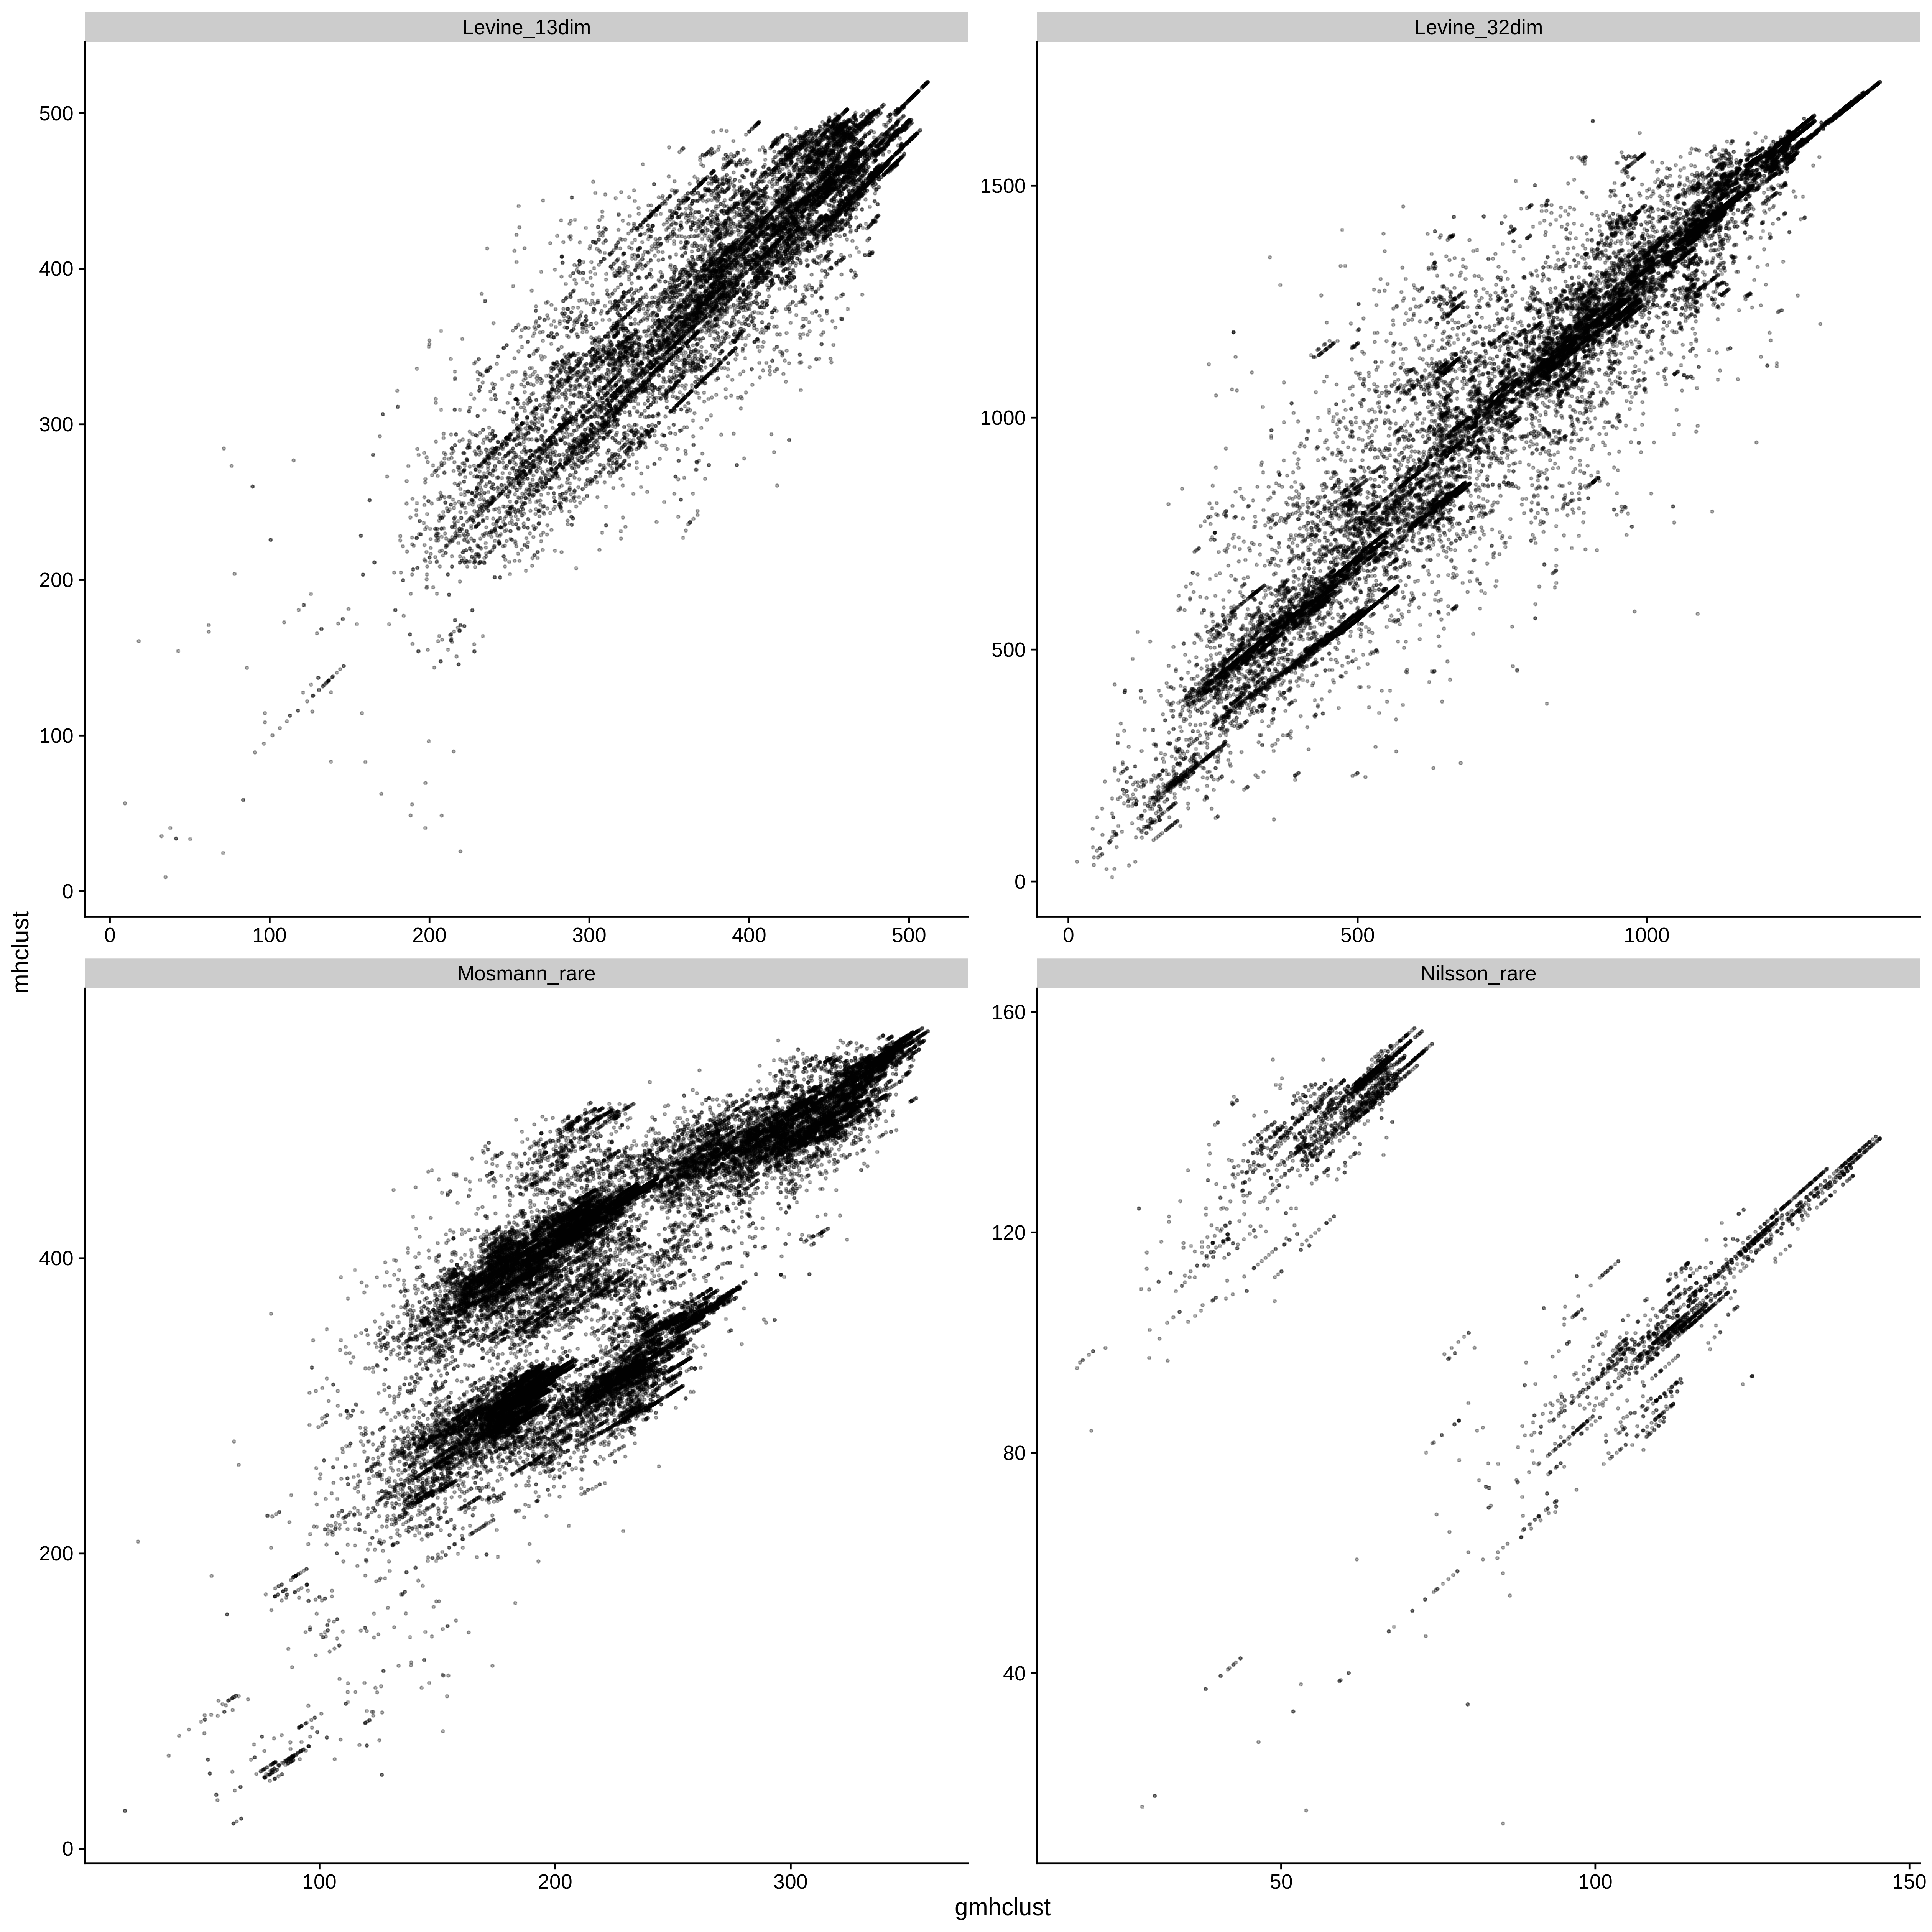
\includegraphics[width=\linewidth]{img/single_result}
	\caption{Plotted point heights of \texttt{gmhclust} and \texttt{mhclust} clusterings of~the~selected single-point datasets. The Mahalanobis threshold was set to default ($\frac{1}{2}$).}
	\label{fig04:single_result}
\end{figure}

\subsection{Apriori dataset results comparison}

We did not down-sample the selected apriori datasets and proceeded the same way as in the previous experiment (see fig.~\ref{fig04:apriori_result}). Here, the experiments showed the~almost straight line. It was expected, as the presence of apriori clusters effectively removed a possible error created during the early algorithm stages where the~implementations differed. More specifically, the propagation of possible clustering differences was stopped when the apriori clusters were completely clustered (as the clusterings aligned at that point).

When all apriori clusters were processed, the GPU and CPU measures of dissimilarity applied on the remaining clusters did not differ as the clusters were big enough. Hence, no other opportunity for possible branching occurred. This experiment also shows the importance of clustering early stages and how it can affect the~whole result.

\begin{figure}\centering
	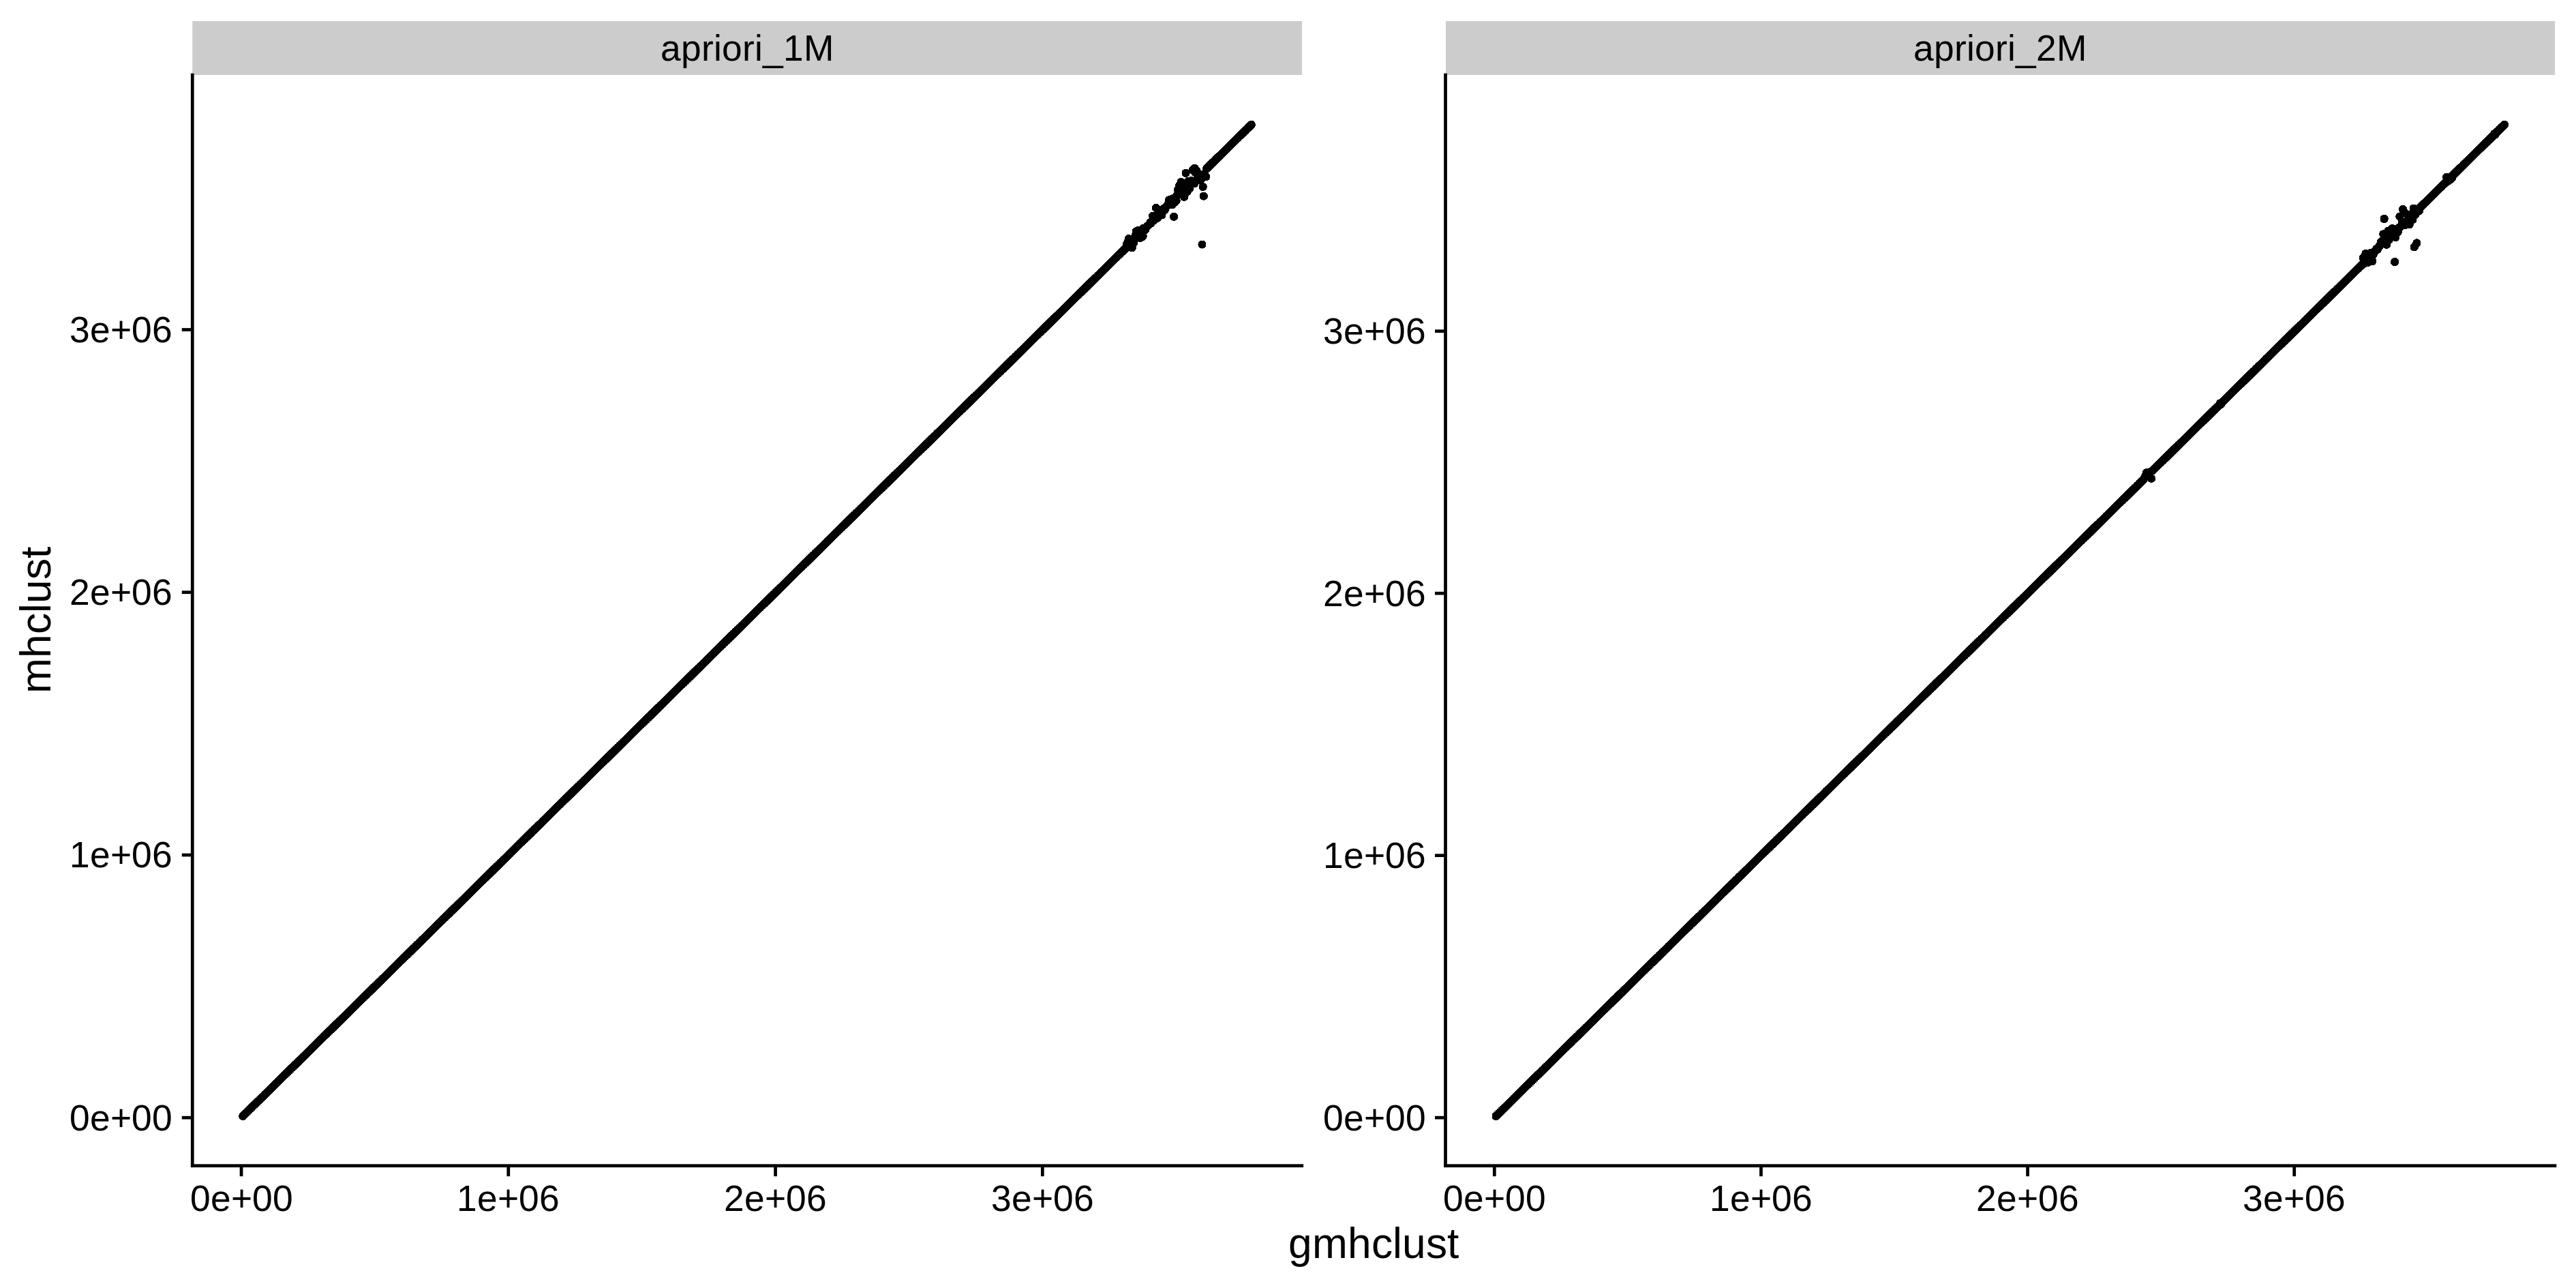
\includegraphics[width=\linewidth]{img/apriori_result}
	\caption{Plotted point heights of \texttt{gmhclust} and \texttt{mhclust} clusterings of~the~selected apriori datasets. The Mahalanobis threshold was set to apriori cluster size.}
	\label{fig04:apriori_result}
\end{figure}



\chapter*{Conclusion}
\addcontentsline{toc}{chapter}{Conclusion}

Over the past years, implementing general clustering algorithms using GPUs has become an expanding topic. As there is always more data to process, GPU implementations help greatly in accelerating a related research.  Still, there are many of~the algorithms that are supported only on CPUs, which can significantly decrease their usability. In the present thesis we have proposed and tested an implementation of the Mahalanobis-average hierarchical clustering analysis accelerated on a single GPU. 

For the proposed implementation, we used CUDA platform to communicate with a GPU. We employed high throughput operations like warp shuffle instructions and utilized a device memory hierarchy using shared and constant memory. With~the~stated features, we have achieved remarkable performance improvements.

The proposed MHCA implementation provides performance increase of up to 5000x in measured single-point datasets and 20x in apriori datasets. Moreover, it requires only linear space with respect to the dataset size, which is an~important factor in the general clustering scalability.

With such performance increase, this implementation is able to extend the size of reasonably computable datasets from hundreds of thousands to millions of points. It can be used to advance research in the field of cell cytometry by~decreasing computation time as well as enabling to compute larger datasets.

\subsection*{Future work}

The experiments showed that the measure of dissimilarity between small clusters may be too naive and can propagate a creation of unwanted clusters. This weakness can be addressed by implementing a different dissimilarity measure for clusters under the Mahalanobis threshold. For example, we can perform a transformation on a covariance matrix of a small cluster to make it regular. Then it can be properly inverted and used in the Mahalanobis distance formula.

Moreover, a covariance matrix can be normalized by dividing each element by its discriminant. When used in the distance formula, this transformation produces the combination of the Mahalanobis and Euclidean distance.

The work can be further expanded by implementing the Full Mahalanobis distance (see def.~\ref{def01:fmd}). It can cover the cases when CMD does not provide precise dissimilarity measure which can lead to a better clustering results. Naturally, it would come for the price of~a~greater overall time complexity. 

%%% Bibliography
%%% Bibliography (literature used as a source)
%%%
%%% We employ bibTeX to construct the bibliography. It processes
%%% citations in the text (e.g., the \cite{...} macro) and looks up
%%% relevant entries in the bibliography.bib file.
%%%
%%% The \bibliographystyle command selects, which style will be used
%%% for references from the text. The argument in curly brackets is
%%% the name of the corresponding style file (*.bst). Both styles
%%% mentioned in this template are included in LaTeX distributions.

\bibliographystyle{plainnat}    %% Author (year)
% \bibliographystyle{unsrt}     %% [number]

\renewcommand{\bibname}{Bibliography}

%%% Generate the bibliography. Beware that if you cited no works,
%%% the empty list will be omitted completely.

\bibliography{bibliography}

%%% If case you prefer to write the bibliography manually (without bibTeX),
%%% you can use the following. Please follow the ISO 690 standard and
%%% citation conventions of your field of research.

% \begin{thebibliography}{99}
%
% \bibitem{lamport94}
%   {\sc Lamport,} Leslie.
%   \emph{\LaTeX: A Document Preparation System}.
%   2nd edition.
%   Massachusetts: Addison Wesley, 1994.
%   ISBN 0-201-52983-1.
%
% \end{thebibliography}


%%% Figures used in the thesis (consider if this is needed)
%\listoffigures

%%% Tables used in the thesis (consider if this is needed)
%%% In mathematical theses, it could be better to move the list of tables to the beginning of the thesis.
%\listoftables

%%% Abbreviations used in the thesis, if any, including their explanation
%%% In mathematical theses, it could be better to move the list of abbreviations to the beginning of the thesis.
%\chapwithtoc{List of Abbreviations}

%%% Attachments to the master thesis, if any. Each attachment must be
%%% referred to at least once from the text of the thesis. Attachments
%%% are numbered.
%%%
%%% The printed version should preferably contain attachments, which can be
%%% read (additional tables and charts, supplementary text, examples of
%%% program output, etc.). The electronic version is more suited for attachments
%%% which will likely be used in an electronic form rather than read (program
%%% source code, data files, interactive charts, etc.). Electronic attachments
%%% should be uploaded to SIS and optionally also included in the thesis on a~CD/DVD.
%%% Allowed file formats are specified in provision of the rector no. 72/2017.
\appendix
\chapter{User guide}

\section{Build guide}

The Mahalanobis-average hierarchical clustering project was developed with the CMake build tool. To build the executable, use CMake configure and build commands in a build directory. Then, the directory \texttt{para} will contain \texttt{gmhclust} executable. The only dependency is the CUDA compiler (\texttt{nvcc}). The executable should be portable to all platforms supporting \texttt{nvcc}; it was successfully tested on Ubuntu 18.04 and Windows 10. See the following steps:

\begin{lstlisting}
cd gmhc
mkdir build && cd build
cmake ..
cmake --build .
ls para/gmhclust
\end{lstlisting}

\section{Running the program}

The \texttt{gmhclust} executable has three command line parameters:
\begin{enumerate}
	\item \emph{Dataset file path} -- The mandatory parameter with a path to a dataset file. The file is binary and has structure as follows:
	\begin{enumerate}
		\item 4B unsigned integer $D$ -- point \emph{dimension}
		\item 4B unsigned integer $N$ -- \emph{number} of points
		\item $N\cdot D$ 4B floats -- $N$ single-precision $D$-dimensional points stored one after another
	\end{enumerate}
	\item \emph{Mahalanobis threshold} -- An absolute positive number that states the Mahalanobis threshold. It is the mandatory parameter.
	\item \emph{Apriori assignments file path} -- An optional path to an apriori assignments file --- a file with space separated 4B unsigned integers (assignment numbers). The number of integers is the same as the number of points in the dataset; it sequentially assigns each point in the dataset file an assignment number. Then simply, if the $i$-th and the $j$-th assignment numbers are equal, then the $i$-th and $j$-th points are assigned the same apriori cluster. 
\end{enumerate}

The executable writes the clustering process to the standard output. Each line contains an ID pair of merged clusters with their merge distance as well.


\chapter{Enclosed CD}

The enclosed CD contais three folders:

\begin{itemize}
	\item \texttt{gmhc} contains the source code of the implementation.
	\item \texttt{benchmark} contains scripts and a guide how to reproduce some of the performed experiments.
	\item \texttt{docs} contains the program documentation.
\end{itemize} 


\openright
\end{document}
